\documentclass{article}
\usepackage[utf8]{inputenc}
\setlength{\parindent}{0cm}
\addtolength{\hoffset}{-2cm}
\addtolength{\textwidth}{4cm}
\usepackage[frenchb]{babel}
\usepackage[T1]{fontenc}
\usepackage[hidelinks]{hyperref}
\usepackage{graphicx}
\usepackage{afterpage}
\usepackage{minted}
\usepackage{pdflscape}
\usepackage{pdfpages}
\usepackage{amssymb}
\usepackage{amsmath}
\usepackage{float}
\usepackage{fancyhdr}

\pagestyle{fancy}
\fancyhf{}
\fancyhead[LE,RO]{\leftmark}
\fancyfoot[R]{\thepage}
\fancyfoot[L]{Ibanez Thomas}

\newcommand*{\printdate}{%
   \ifcase \month\or Janvier\or Février\or Mars\or Avril\or Mai\or Juin\or Juillet\or Août\or Septembre\or Octobre\or Novembre\or Décembre\fi \space \number\year}

\title{Algorithmes génétiques pour l'intelligence artificielle}
\author{Thomas Ibanez}
\makeindex


\begin{document}

\begin{titlepage}
	\vspace*{-3cm}
		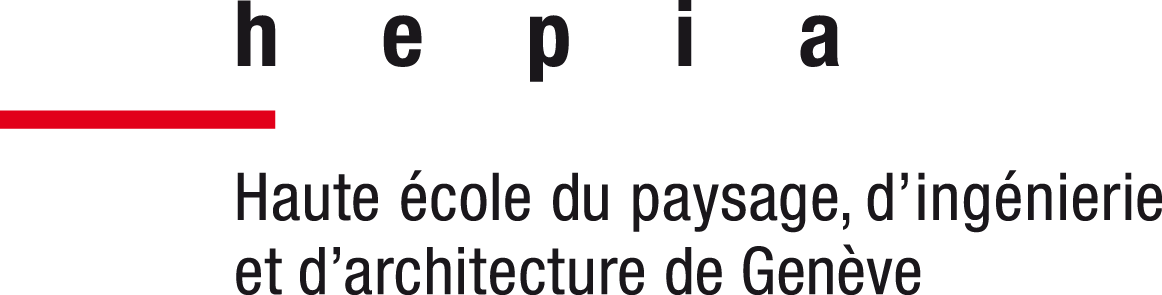
\includegraphics[width=.3\linewidth]{hepia.png}
		\hfill
		
\includegraphics[width=.3\linewidth]{hes.png}\par
	\vspace{1cm}
	\centering
	{\scshape\huge Algorithmes génétiques pour l'intelligence artificielle \par}
	\vspace{1cm}
	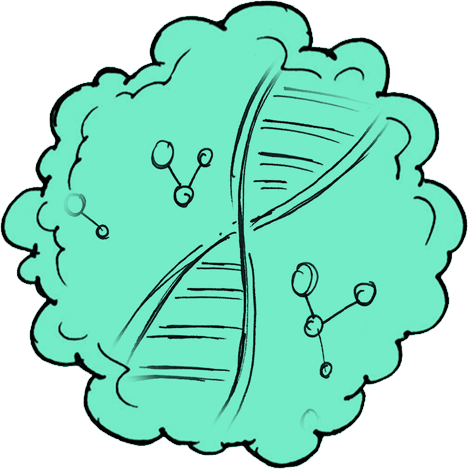
\includegraphics[scale=0.4]{logo.png}\par
	\vspace{1.5cm}
	{\Large\scshape Thèse de bachelor présentée par\par}
	\vspace{0.5cm}
	{\bfseries\Large M. Thomas Ibanez\par}
	\vspace{0.8cm}
	{\scshape\Large Pour l'obtention du titre Bachelor of Science HES-SO en\par}
	\vspace{0.5cm}
	{\bfseries\Large Ingénierie des technologies de l'information avec orientation en Logiciels et Systèmes complexes\par}
	\vfill
	Professeur HES responsable\par
	\bfseries{Orestis Malaspinas\par}

	\vfill

	{\large\ \printdate \par}
\end{titlepage}

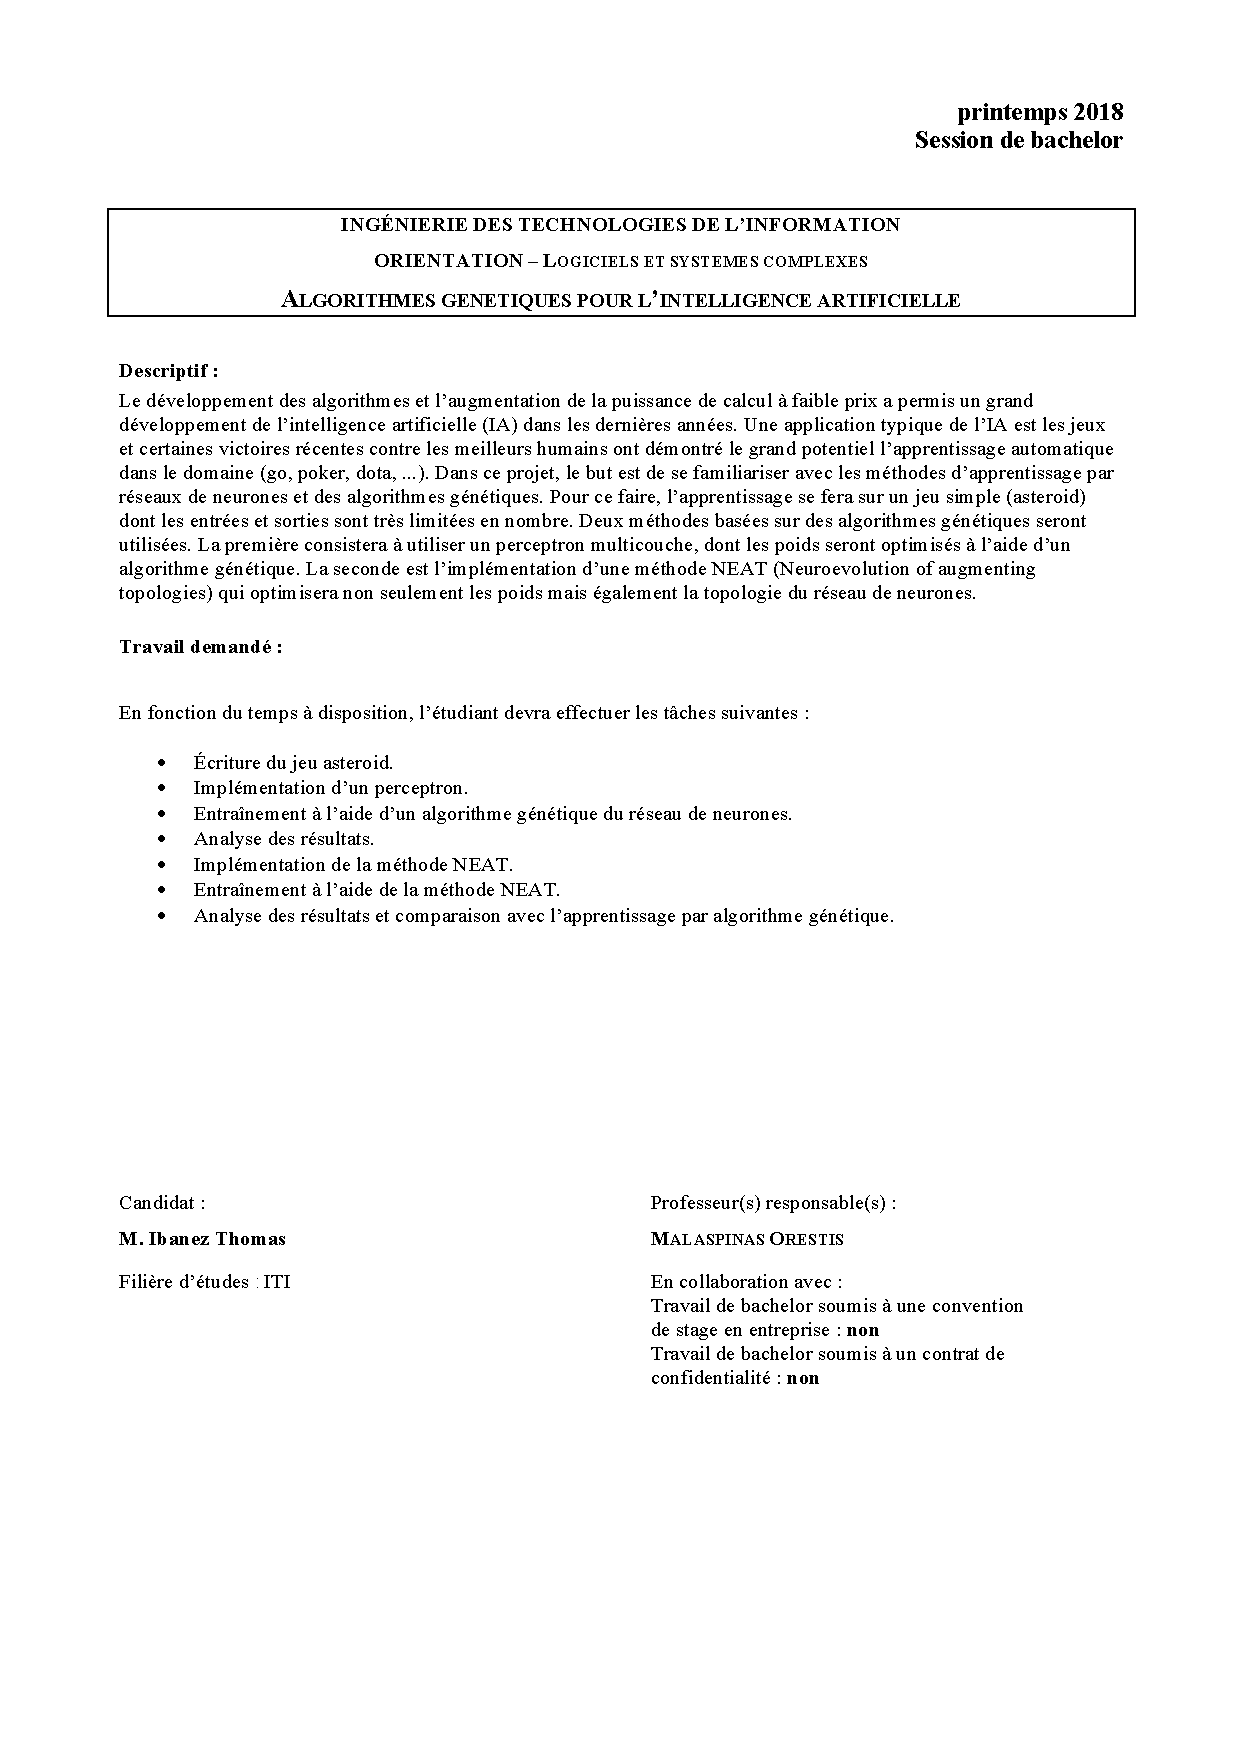
\includepdf[pages=1, offset=2cm 0]{enonce}

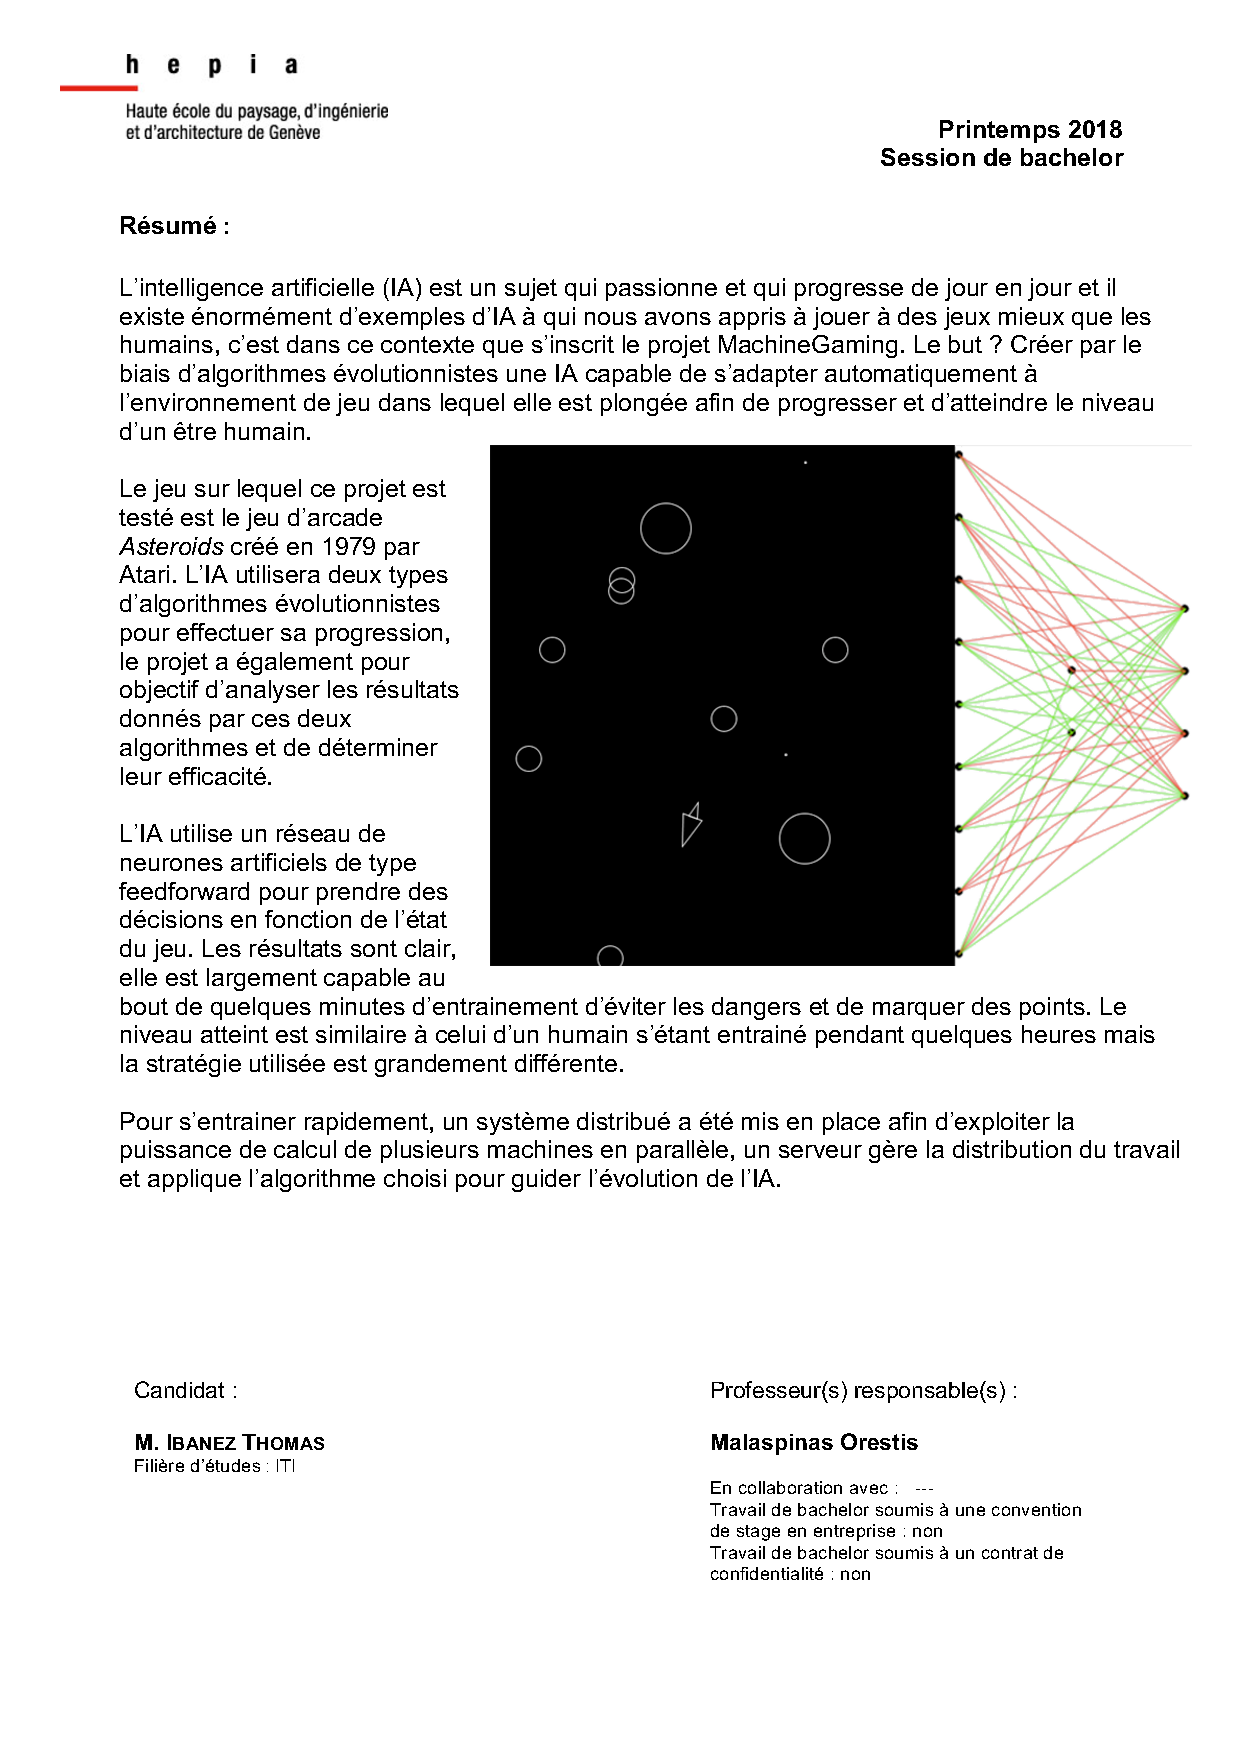
\includepdf[pages=1, offset=2cm 0]{resume}

\section*{Remerciements}

Je tiens à remercier M. Orestis Malaspinas qui m'a aidé et encadré pendant toute la durée de ce projet.\\

Merci aux professeurs de l'hepia et à mes camarades de classe avec qui j'ai passé trois années extrêmement enrichissantes.\\

Je remercie également les membres de ma familles ainsi que mes amis qui m'ont aidé et soutenu durant le réalisation de ce travail.\\

Finalement, merci à M. Natanaël Nufer avec qui j'ai pu échanger sur le domaine de l'intelligence artificielle tout au long de la réalisation de ce projet.
\newpage
\section*{Acronymes}
\begin{itemize}
	\item \textbf{IA} = Intelligence artificielle.
	\item \textbf{NEAT} = Neuroevolution of Augmenting Topologies.
	\item \textbf{MLP} = Multilayer Perceptron (Perceptron Multicouches).
	\item \textbf{TLV} = Type, Longueur, Valeur.
	\item \textbf{API} = Application Programming Interface.
	\item \textbf{JSON} = JavaScript Object Notation
	\item \textbf{CNN} = Convolutional Neural Network
	\item \textbf{RNN} = Recurrent Neural Network
\end{itemize}

\newpage
\tableofcontents

\newpage

\listoffigures

\newpage

\section{Introduction}

Ces dernières années, l'apprentissage automatique (Machine Learning) a pris une place très importante dans le monde de l'informatique et nous avons pu assister aux prouesses accomplies par des intelligences artificielles tels que la victoire d'AlphaGo face à Lee Sedol au jeu de Go en 2016\cite{wikialphagolee}. Cet événement n'est pas sans rappeler la défaite de Kasparov contre Deep Blue en 1997 qui avait défrayé le chronique\cite{kasparov}.\\
Mais comment en sommes nous arrivés là, et quels sont les techniques qui se cachent derrière ces impressionnants résultats ?\\
Il y a plusieurs manières de faire du machine learning ; une des plus populaire, celle qui est utilisée pour ce travail, est le réseau de neurones artificiels. Cette technologie existe depuis bien longtemps, mais ce sont les récents progrès en terme de puissance de calcul qui ont amorcé sa montée comme technologie phare du domaine\cite{nnpower}.\\

La méthode classique pour entrainer des réseaux de neurones est la rétropropagation du gradient (backpropagation). Cette technique consiste à comparer les résultats obtenus aux résultats attendus afin de corriger le réseau de neurones petit à petit jusqu'à atteindre le résultat désiré. Le désavantage est qu'il faut avoir à sa disposition un grand nombre d'entrées dont nous connaissons la nature afin de pouvoir les comparer aux résultats du réseau. Par exemple, il existe une base de données de chiffres écrit à la main avec leur valeur réelle sur \url{http://yann.lecun.com/exdb/mnist/} (70'000 entrées).\\

Cependant, générer une telle base de données est un travail énorme, ainsi ces dernières années nous avons assisté à l'émergence de nouvelles techniques ne nécessitant pas d'exemples.\\

Une de ces techniques, qui a été utilisée pour l'apprentissage d'AlphaGo\cite{alphago}, est l'apprentissage par renforcement (Reinforcement learning). Cette méthode consiste à juger les décisions prises par un agent autonome en lui donnant une récompense positive ou négative afin que l'agent, au fur et à mesure des expériences trouve une stratégie optimale\cite{wikirl}. Cette façon de faire peut être comparée au comportement d'un enfant qui apprend à faire du vélo. Quand il tombe il va avoir mal, c'est une récompense négative. Il va donc corriger son comportement de façon à ne plus tomber. A l'inverse, quand il arrive à aller loin, il va être fier et donc favoriser ce comportement, c'est une récompense positive.\\

Cependant il existe une méthode encore plus généraliste pour l'apprentissage: la neuroévolution. Cette méthode se base sur les algorithmes évolutionnistes dont le fonctionnement est inspiré de la sélection naturelle qui a guidé l'évolution de la vie sur terre. En effet, à partir d'un ensemble d'organismes que nous allons évaluer à leur capacité à effectuer une tâche donnée, ce que nous appelons le \textit{fitness} de l'organisme, nous allons sélectionner les meilleurs d'entre eux afin de les faire se "reproduire" pour créer la génération suivante qui sera à son tour évaluée et nous recommencerons ce processus autant de fois que nécessaire\cite{wikineuroevolution}.\\

Le but de ce travail de bachelor est d'étudier et de comparer le comportement de deux algorithmes de neuroévolution en analysant la faculté de chacun à apprendre à jouer à des jeux vidéo. Cette technique à été choisie car elle permet un développement plus libre de l'IA en ne jugeant que le résultat et non pas les actions qui y mènent.\\

Ce travail est structuré comme suit: Dans le chapitre 2, nous parlerons de la notion d'agent intelligent et d'environnement.\\
Dans le chapitre 3 nous verrons le fonctionnement des réseaux de neurones artificiels et les méthodes permettant de les entraîner.\\
Dans le chapitre 4 nous verrons ce qu'est un algorithme évolutionniste et les concepts de bases sur lesquels ce type d'algorithme se repose.\\
Dans le chapitre 5 nous palerons d'un algorithme naïf permettant de faire évoluer un réseau de neurones à topologie fixe, cet algorithme utilise de manière directe les concepts vus dans le chapitre 4.\\
Dans le chapitre 6 nous verrons l'algorithme NEAT, cet algorithme utilise également les concepts discutés dans le chapitre 4 mais il en ajoute également de nouveaux.\\
Dans le chapitre 7 nous parlerons l'implémentation du projet et l'architecture réseau qui a été produite.\\
Dans le chapitre 8 nous verrons le fonctionnement de l'interface de contrôle qui va nous permettre d'utiliser le système pour entraîner des réseaux de neurones à jouer à des jeux-vidéo.\\
Dans le chapitre 9 nous aurons un aperçu du système de gestion de base de données mis en place pour enregistrer / charger des tâches.\\
Dans le chapitre 10 nous parlerons de l'API mise en place pour le contrôle du système.\\
Dans le chapitre 11 nous verrons le jeu implémenté et les résultats obtenu.\\
Finalement dans le chapitre 12 nous conclurons ce travail et verrons les potentielles suites possibles.
\newpage

\section{Agent Intelligent}

Dans ce chapitre nous abordons la notion d'agent intelligent et les concepts qui entourent cette notion. Cette notion est essentielle car l'objectif de ce travail est de créer le meilleur agent possible.

\subsection{Définition}

Un agent intelligent est une entité autonome qui observe son environnement grâce à des capteurs et qui peut agir sur l'état de son environnement grâce à des effecteurs. Cette entité doit avoir un objectif (gagner une partie de Go par exemple), elle peut également apprendre ou utiliser ses connaissances pour atteindre son but\cite{wikiia}.\\

\begin{figure}[H]
\begin{center}
	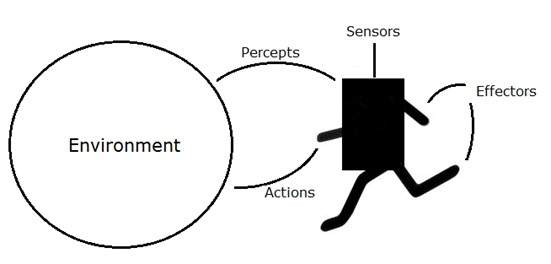
\includegraphics[scale=0.5]{agent_environment.jpg}
	\caption{Illustration d'un agent}
\end{center}
\end{figure}

\subsection{Mesure de la performance}

La mesure de la performance est un critère qui va définir l'efficacité d'un agent, ce critère dépend évidement de la tâche demandée à l'agent. Cette mesure est analogue à la mesure de la valeur sélective (fitness) d'un organisme en biologie. Ainsi, si le tâche demandée à l'agent est de séparer les M\&M's bleus des M\&M's rouges, sa performance peut être mesurée par son taux d'erreur et sa rapidité.

\subsection{Rationalité}

La rationalité est le fait d'être raisonnable, sensible et d'avoir un bon sens du jugement.\\
Un agent rationnel va toujours effectuer la "bonne" action, celle qui va apporter le plus de succès à l'agent par rapport à la séquence perçue\cite{tutoptai}. Le but de tout développement d'agent intelligent est donc de créer un agent rationnel afin qu'il soit aussi performant que possible.

\subsection{Environnement}

L'environnement peut être de différentes natures en fonction du problème pour lequel l'agent est déployé. Les différents types d'environnement sont expliqués ci-dessous.

\subsubsection{Discret / Continu}

Si les états possibles de l'environnement sont dénombrables et clairement définis, l'environnement est dit "discret". Par exemple, le jeu de Go est un environnement discret car nous pouvons lister tout les états possibles du plateau. En revanche, un simulateur de conduite est continu, nous ne pouvons pas lister toutes les positions possibles de la voiture\cite{tutoptai}.

\subsubsection{Observable / Partiellement Observable}

L'environnement est observable si l'agent peut à tout moment en observer la totalité, sinon l'environnement est partiellement observable. Par exemple le jeu DotA 2 n'est que partiellement observable car du brouillard cache une partie de l'environnement contrairement au jeu de Go où les deux joueurs voient la totalité du plateau de jeu\cite{tutoptai}.

\subsubsection{Statique / Dynamique}

Si l'environnement ne change pas tant qu'un agent n'agit pas il est dit statique, sinon il est dynamique. Un exemple d'environnement statique est le jeu du monopoly, tant qu'un joueur n'agit pas l'état du jeu ne change pas. Au contraire dans les flippers, la balle va continuer à bouger même si le joueur ne fait rien\cite{tutoptai}.

\subsubsection{Simple agent / Multi-agents}

Lorsque l'environnement n'est influencé que par un seul agent il est dit simple agent, c'est la cas du jeu space invaders qui se joue seul. Si l'environnement est influencé par plusieurs agents il est dit multi-agents, la planète terre est donc un environnement multi-agents\cite{tutoptai}.

\subsubsection{Déterministe / Non-déterministe}

L'environnement est dit déterministe si nous pouvons prévoir, à partir d'une observation de l'état actuel de l'environnement, l'état suivant de l'environnement. Autrement dit si l'aléatoire n'intervient pas dans l'évolution de l'environnement alors il est déterministe\cite{tutoptai}. Le jeu d'échecs est déterministe car aucuns événement aléatoire ne vient perturber le plateau, au contraire un jeu comme pac-man est non-déterministe car le chemin pris par les fantômes qui chassent le joueur est en partie déterminé aléatoirement.

\subsubsection{Épisodique / Non-épisodique}

Un environnement épisodique est divisé en épisodes, un épisode est une série d'observation qui mène à une et une seule action, une fois l'action effectuée, l'épisode est terminé. Ainsi les actions et décisions passée de l'agent (les épisodes passées) n'ont aucune influence sur l'état actuel de l'environnement.\\
Un exemple d'environnement épisodique est un agent qui regarde des images pour les classer, une fois le choix fait celui-ci n'aura pas d'influence sur les images suivantes. Au contraire dans un jeu comme le jeu d'échecs, chaque coup dépend du coup précédent, c'est donc un environnement non-épisodique\cite{tutoptai}.

\newpage
\section{Réseau de Neurones Artificiels}

Cette section va expliquer la notion de réseau de neurones artificiels, de leur origine et leur lien avec la biologie jusqu'aux différentes manières de les entraîner. Cette technologie est devenue incontournable dans le domaine de l'intelligence artificielle tant ils ont réalisé de prouesses ces dernières années.

\subsection{Définition}

Un réseau de neurones est un modèle, inspiré du fonctionnement du cerveau humain, qui va consister en un ensemble de neurones artificiels (aussi appelés perceptrons), disposés en couches qui vont communiquer en propageant une information\cite{wikiann}. En effet, les neurones de notre cerveau vont collecter les signaux en provenance de leurs dendrites, puis si les signaux sont assez forts envoyer une impulsion le long de leur axone vers les neurones suivants qui vont faire de même. A noter que les connexions entre deux neurones peuvent être plus ou moins fortes (le signal va donc se propager avec une intensité variable)\cite{neuronswork}.

\begin{figure}[H]
\begin{center}
	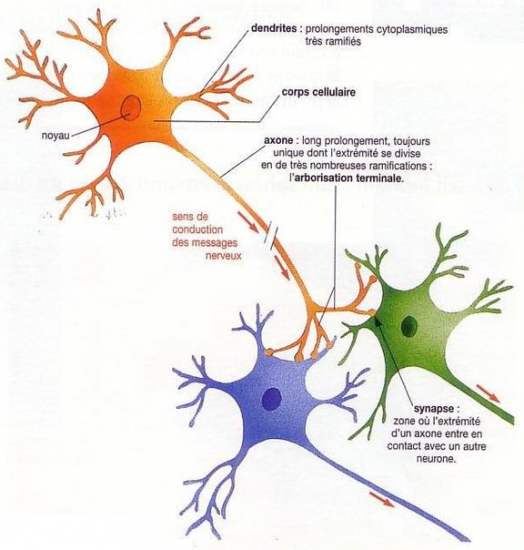
\includegraphics[scale=0.5]{neurones.png}
	\caption{Représentation des neurones dans le cerveau humain \cite{neurons}}
\end{center}
\end{figure}

Les perceptrons quant à eux vont imiter (de manière simplifiée) ce comportement, chaque perceptron va prendre le signal envoyé par chacun de ses voisins de la couche précédente, puis multiplier cette valeur par le poids de la connexion et finalement faire la somme de toutes les valeurs pondérées. Cette somme est ensuite passée dans une fonction (dites fonction d'activation) qui va la placer dans un intervalle (entre 0 et 1 par exemple) et renvoyer le résultat à tous ses voisins de la couche suivante qui vont faire de même\cite{wikiperceptron}.

D'un point de vue mathématique le comportement d'un perceptron peut être écrit comme:
\begin{equation}
o = f(\sum_{i=1}^{n} \vec{S_i} \cdot \vec{W_i})
\label{eq:percep}
\end{equation}

Cette opération peut être simplifiée en utilisant le produit scalaire:

\begin{equation}
o = f(\vec{S} \cdot \vec{W})
\end{equation}

Où\\
$o$ est le signal qui va sortir du perceptron\\
$f$ est la fonction d'activation\\
$n$ est le nombre de voisins de la couche précédente\\
$\vec{S}$ est le vecteur des signaux des voisins la couche précédente\\
$\vec{W}$ est le vecteur des poids entre le perceptrons et ses voisins de la couche précédente

\begin{figure}[H]
\begin{center}
	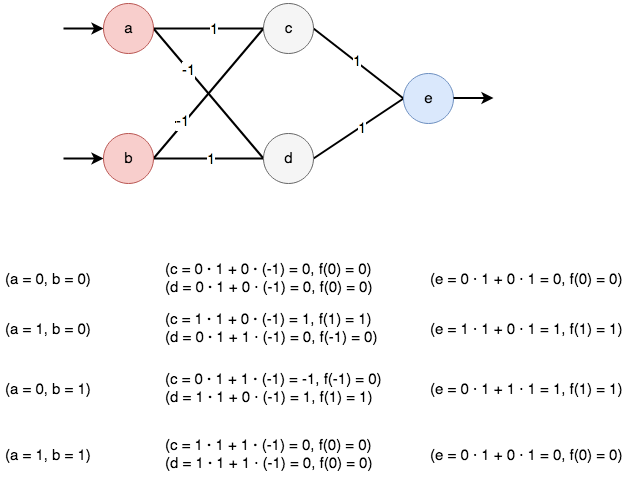
\includegraphics[scale=0.6]{xor.png} 
	\caption{Porte logique "ou exclusif" (XOR) simulée par un réseau de neurones}
\end{center}
\end{figure}

Les neurones de la première couche vont recevoir leur valeur depuis l'extérieur. Ces entrées (aussi appelées \textit{features}) dépendent du problème pour lequel le réseau est employé. Ainsi si nous cherchons à prédire la note d'un examen en fonction du temps de révision et du nombre d'heures de sommeil, les entrées du réseau seront le temps de révision et le nombre d'heures de sommeil.\\
 Chaque neurone de la couche suivante calculera sa valeur par propagation du signal de la couche précédente afin d'arriver jusqu'à la dernière couche de neurones qui déterminera la prédiction du réseau de neurones. Cette prédiction est également appelée \textit{label}. Dans le cas de notre exemple, le label du réseau sera la note prévue.\\
 Avant de pouvoir utiliser notre réseau pour faire des prédictions, il faut l'entrainer, c'est à dire ajuster les paramètres (poids, topologie) afin que les labels soient le plus correct possible pour des features données.\\
 
 Les réseau de neurones possèdent également une entrée particulière, dont la valeur sera toujours le maximum selon l'interval de fonctionnement, cette entrée est appelée le biais (bias en anglais). Dans les figures suivantes je ne représenterai pas le biais pour alléger la lecture.
 
\begin{figure}[H]
\begin{center}
	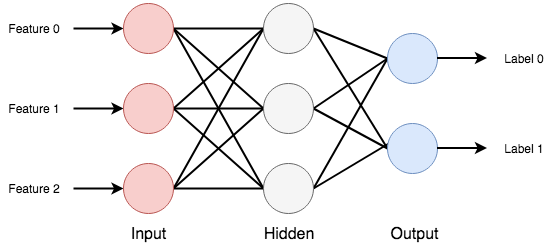
\includegraphics[scale=0.7]{ff.png}
	\caption{Réseau de neurones}
\end{center}
\end{figure}
 
 Il est cependant important de ne pas mystifier le fonctionnement des réseaux de neurones. Ce sont certes des "boites noires", c'est à dire qu'il n'est pas possible d'analyser un réseau et d'expliquer pourquoi une connexion donnée a un tel poids. En revanche, il ne faut pas perdre de vue que leur comportement est exprimable par une fonction mathématique. En effet tout comme le comportement d'un perceptron est décrit dans l'équation \ref{eq:percep} le comportement de n'importe quel réseau de neurones peut-être décrit par une equation dépendant du réseau.

\subsection{Apprentissage supervisé}

L'apprentissage supervisé est une manière d'entrainer un réseau de neurones avec un ensemble de couples (features, labels). Le but est de commencer avec un réseau initialisé aléatoirement, puis de lui donner en entrée des features dont les labels sont connus et de comparer les labels donnés par le réseau aux labels attendus.\\
En fonction du taux d'erreur, il sera possible de corriger les poids des connexions du réseau pour minimiser ce taux\cite{wikisupervised}.\\

Les avantages principaux de cette technique d'apprentissage sont la rapidité d'entraînement et la justesse atteignable étant donné que le fonctionnement ne dépend pas d'heuristiques.\\

Les désavantages sont le temps de génération de la base d'exemples et le fait qu'il faille connaitre le label attendu pour chaque feature (nous savons à coup sûr qu'une image de chien doit être classifiée comme "chien" mais nous ne savons pas le coup idéal à jouer selon l'état d'un plateau de jeu). Le problème du sur-apprentissage (overfitting) intervient également, la conséquence du sur-apprentissage est que le réseau va analyser de manière trop exacte les données de son ensemble d'exemples en faisant des lien de causalité qui n'ont pas lieu d'être et va ensuite faire des erreurs lorsqu'il devra classer des nouvelles données.

\subsection{Apprentissage non supervisé}

L'apprentissage non supervisé est une méthode d'apprentissage où l'entraînement se fait avec un semble de features dont le label n'est pas connu. Une utilisation de cette technique est le partitionnement de données où le réseau va apprendre à regrouper des features similaires dans la même catégorie\cite{wikiunsupervised}.\\

Cette méthode peut être comparée à la manière dont un enfant apprend à reconnaître son environnement. Si il voit 50 voitures, il va pouvoir les associer comme étant des objets similaires, sans pour autant qu'on ait eu besoin de lui expliquer ce qu'est un voiture.

\subsection{Apprentissage par renforcement}

L'apprentissage par renforcement intervient lorsqu'on veut optimiser les décisions prises par un agent intelligent en fonction de son environnement. Il est possible que l'agent soit controlé par un réseau de neurones, dans ce cas, les décisions seront les labels et les informations sur son environnement seront les features. Le concept de l'apprentissage par renforcement est de récompenser ou de pénaliser les choix fait par l'agent afin qu'au fur et à mesure des expériences il optimise son comportement\cite{wikirl}.

\subsection{Neuroévolution}

La neuroévolution est une technique d'entraînement dont le but est d'utiliser les principes des algorithmes évolutionnistes afin d'optimiser un réseau de neurones pour effectuer la tâche désirée. A la différence de l'apprentissage par renforcement, ce ne sont pas les actions individuelles qui vont être jugées mais l'efficacité totale du réseau. Nous ne cherchons donc pas à développer un comportement particulier mais juste à être plus optimal, le choix de la stratégie pour atteindre son but est laissée au réseau de neurones\cite{wikineuroevolution}.\\

\subsection{Fonctions d'activation}

Les fonctions d'activation sont des fonctions qui ont pour tâche de limiter la valeur des neurones dans un intervalle donné. Afin de pouvoir appliquer la rétropropagation du gradient il faut également que la fonction soit dérivable.
Voici quelques exemples de fonctions utilisées couramment:\\

La sigmoid $\sigma : \mathbb{R} \rightarrow ]0, 1[$
\begin{equation}
	\sigma : x \mapsto \frac{1}{1 + e^{-\beta x}}
\end{equation}

\begin{figure}[H]
\begin{center}
	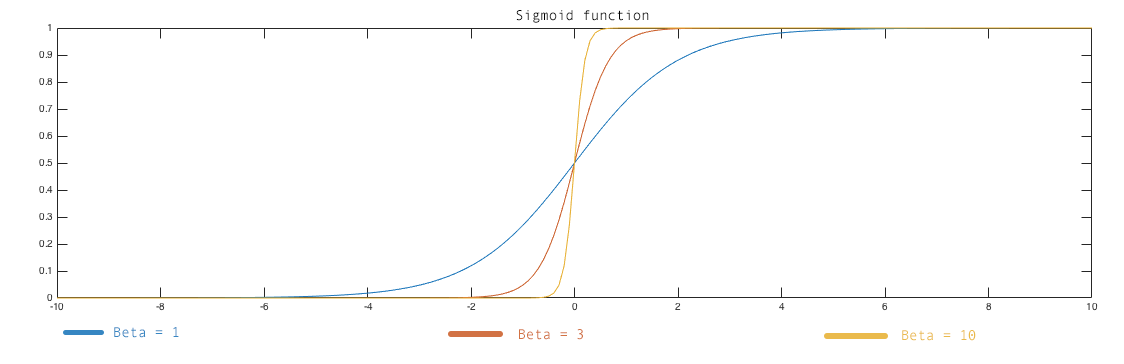
\includegraphics[scale=0.4]{sigmoid.png} 
	\caption{Fonction Sigmoid avec des $\beta$ variables}
\end{center}
\end{figure}

La tangente hyperbolique $tanh : \mathbb{R} \rightarrow ]-1, 1[$
\begin{equation}
	tanh : x \mapsto \frac{e^x - e^{-x}}{e^x + e^{-x}}
\end{equation}

\begin{figure}[H]
\begin{center}
	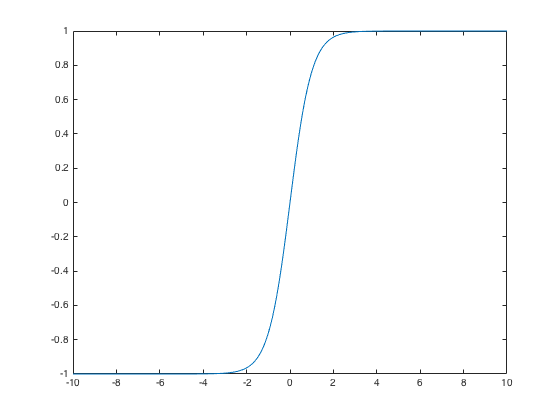
\includegraphics[scale=0.4]{tanh.png} 
	\caption{Fonction tangente hyperbolique}
\end{center}
\end{figure}

La fonction step $step : \mathbb{R} \rightarrow [0, 1]$
\begin{equation}
	step : x \mapsto
		\begin{cases}
			0, & \text{if}\ x \leq 0\\
			1, & \text{otherwise}
		\end{cases}
\end{equation}

\begin{figure}[H]
\begin{center}
	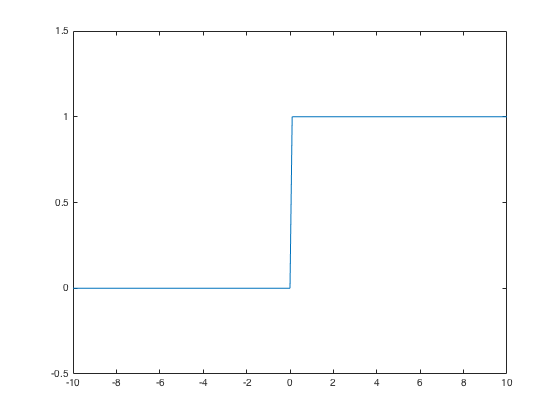
\includegraphics[scale=0.4]{step.png} 
	\caption{Fonction step}
\end{center}
\end{figure}

\newpage
\section{Algorithmes évolutionnistes}

Ce chapitre parle des algorithmes évolutionnistes, nous allons voir leur fonctionnement général et les concepts essentiels qui permettent ce fonctionnement.

\subsection{Définition}

Un algorithme évolutionniste est un algorithme d'optimisation métaheuristique qui cherche, par un processus inspiré de la sélection naturelle, une solution optimale à un problème. Ces algorithmes utilisent des iterations stochastiques pour arriver à maximiser une fonction évaluant leurs performances, dite fonction de fitness\cite{wikiea}.\\

Les sections suivantes expliquent de manière générale les différents points clef de ces algorithmes.

\subsection{Génome \& Phénome}

Le génome est l'ensemble du matériel génétique d'un individu, celui-ci contient toutes les informations nécessaires à la création de l'individu\cite{wikigenome}. Chez les humains le génome est organisé en 23 paires de chromosomes. A partir de ces chromosomes, qui sont uniques à chaque organisme, nous pouvons créer le phénome.\\
Le phénome est l'ensemble de tout les traits observables chez un individu (p.ex la couleur des yeux, de la peau, des cheveux, etc...)\cite{wikiphenome}.\\

Dans le cadre de la neuroévolution, le génome est un encodage refermant les différents paramètres du réseau de neurones tels que les poids des connexion et le topologie du réseau. En décodant le génome il est donc possible de construire le phénome, un réseau de neurones dans notre cas.

\subsection{Population initiale}

La base d'un algorithme évolutionniste est la population initiale. Celle-ci doit être générée aléatoirement afin de représenter un vaste spectre de possibilités. 
Nous ne retrouverons dans cette population aléatoire aucun individu capable d'accomplir parfaitement la tâche demandée, mais certains auront des comportements qui les aideront à obtenir un fitness plus élevé que leurs voisins. C'est donc ceux-ci vont donc passer leurs caractéristiques à la génération suivante par le processus de sélection naturelle.

\subsection{Sélection}

La sélection est un concept essentiel dans l'utilisation d'algorithmes évolutionnistes. L'objectif est de privilégier, en tenant compte du fitness, les individus les plus performants afin qu'ils soient plus souvent sélectionnés pour être parents. Ainsi, les caractéristiques qui les rendent plus performants seront plus largement passés à la génération suivante alors que les caractéristiques des individus plus faibles disparaîtront rapidement\cite{wikifps}.

\begin{figure}[H]
\begin{center}
	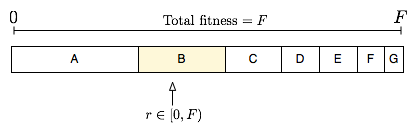
\includegraphics[scale=0.6]{fps.png} 
	\caption{Exemple de sélection proportionnelle au fitness, soit r une variable aléatoire tirée entre 0 et $\phi$, il y a plus de chance que celle-ci sélectionne un organisme plus performant (A, B) qu'un organisme faible (F, G)\cite{wikifps}}
\end{center}
\end{figure}

Les organismes sélectionnés vont donc pouvoir mélanger leurs gènes pour créer des enfant héritants des caractéristiques qui ont rendu leurs parents performants. Ce mélange est fait par l'opération de crossover.

\subsection{Crossover}

Un crossover (ou enjambement en français) est une opération génétique qui consiste à croiser les gènes de deux parents afin de créer le gène de l'enfant. Ce dernier va donc hériter de certaines caractéristiques de l'un où l'autre parent. Un exemple visible de cette opération chez les humains est que l'on reconnait des traits (couleur de peau, yeux, cheveux) des parents chez les enfants\cite{wikicrossover}.\\

Le crossover va donc permettre un mélange de gènes forts dans le but de créer des enfant meilleurs que leurs parents, cependant le crossover ne va pas permettre l'apparition d'innovations ou de comportements nouveaux. C'est pour cette raison que cette opération va de paire avec la mutation.

\subsection{Mutation}

Les mutations sont des événements aléatoires qui vont altérer le génome de façon à créer une innovation, qui va par exemple se traduire par un comportement différent du génome. Dans certains cas les mutations seront bénéfiques (p.ex la capacité à respirer hors de l'eau), dans d'autre la mutation causera un comportement désavantageux (p.ex malformation des membres)\cite{wikimutation}.\\

L'utilisation de mutations dans les algorithmes génétiques va permettre l'apparitions de nouveaux comportements qui peuvent être avantageux pour l'obtention d'une solution optimale. Cependant les mutations pouvant aussi être désavantageuses, il est important de conserver les meilleurs solutions de chaque itération grâce au principe d'élitisme.

\subsection{Elitisme}

L'élitisme est un concept qui va permettre la survie des meilleurs individus d'une génération vers la génération suivante sans que leur code génétique soit modifié\cite{elitism}.\\
La raison pour laquelle ce concept est mis en place est que les solutions optimales trouvées ne doivent pas être perdues à cause de mutations désavantageuses.

\newpage
\section{Evolution du perceptron multicouche - Algorithme Naïf}

Cette section détaille le fonctionnement de l'algorithme évolutionniste mis en place pour faire évoluer les perceptrons multicouches à topologie fixe. Celui-ci va donc uniquement faire varier les poids des connexions dans le réseau pour optimiser son comportement. L'algorithme a été créé en s'inspirant des concepts d'algorithmes évolutionnistes décrits précédemment.

\subsection{Génome \& Phénome}

Pour cet algorithme le génome est simplement la liste des poids constituant le réseau de neurones. Ainsi, étant donné que la topologie du réseau est fixe, nous pouvons le reproduire à l'identique en assignant les bons poids.\\

Le phénome dans le cas de cet algorithme sera un réseau de neurones à topologie fixe et entièrement connecté (Chaque neurone d'une couche donnée est connecté a chaque neurone de la couche suivante).\\

Le réseau de neurones utilise la fonction d'activation Sigmoid avec $\beta = 3$.

\begin{figure}[H]
\begin{center}
	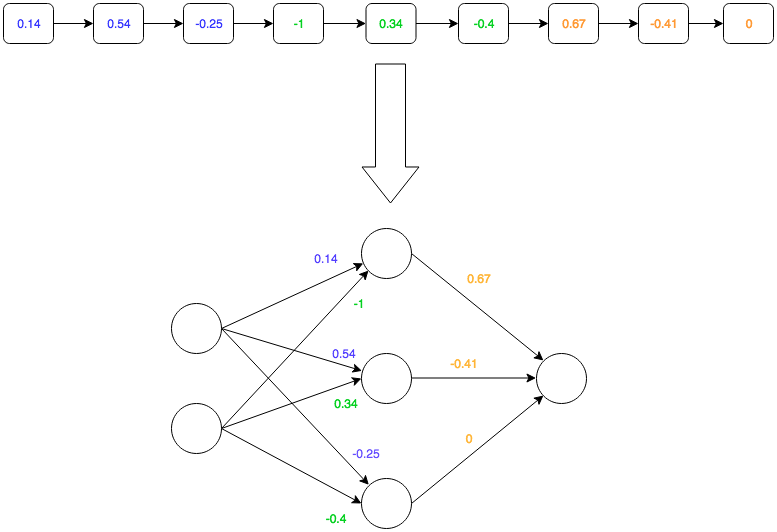
\includegraphics[scale=0.5]{genomephenome.png}
	\caption{Passage du génome au phénome}
\end{center}
\end{figure}

\subsection{Population initiale}

La population initiale est un ensemble de perceptrons multicouche dont la topologie est la même. Les poids entre les couches sont assignés aléatoirement à une valeur entre -1 et +1 afin de représenter un spectre de possibilités aussi large que possible.
\begin{figure}[H]
\begin{center}
	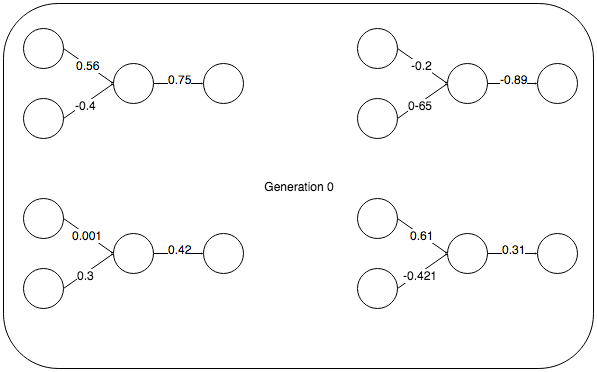
\includegraphics[scale=0.6]{gen0mlp.png} 
	\caption{Exemple de population initiale}
\end{center}
\end{figure}

\subsection{Sélection}

La sélection est utilisée pour choisir un individu de la génération précédente qui va soit passer ses gènes directement (être cloné), soit faire un crossover avec les gènes d'un autre individu lui aussi sélectionné. La probabilité de l'une ou l'autre de ces actions est de 50\%.\\
Le génome résultant de cette sélection subira ensuite une potentielle mutation. Ce processus est répété autant de fois que nécessaire pour créer une nouvelle génération contenant autant d'organismes que la précédente.

\subsection{Crossover}

Le crossover fonctionne d'après un principe très simple:\\
\begin{itemize}
\item Choisir un point de croisement
\item Assigner à l'enfant tous les gènes qui précèdent ce point depuis le premier parent
\item Assigner à l'enfant tous les gènes qui suivent ce point depuis le second parent
\end{itemize}

\begin{figure}[H]
\begin{center}
	\includegraphics[scale=0.6]{"crossover.png"} 
	\caption{Fonctionnement d'un crossover}
\end{center}
\end{figure}

Ainsi, les traits permettant une meilleure survie vont rapidement se répandre dans la population car les individus ayant obtenu un meilleur fitness seront plus souvent sélectionnés pour faire une crossover avec un autre individu.

\subsection{Mutation}

Dans le cas de cet algorithme, étant donné que la topologie est fixe, la mutation sera simplement une variation aléatoire d'un poids dans le réseau de neurones. Ainsi chaque enfant de chaque génération aura 10\% de chance que l'un de ses gènes subisse une mutation.\\
Le poids subira donc une variation d'une valeur aléatoire choisie entre +0.5 et -0.5 cependant le poids sera ensuite fixée dans l'intervalle $[-1, 1]$.

\begin{figure}[H]
\begin{center}
	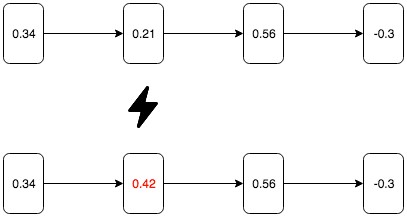
\includegraphics[scale=0.6]{mutation.png}
	\caption{Exemple de mutation dans un génome}
\end{center}
\end{figure}

\subsection{Elitisme}

Pour cet algorithme, seul le champion de la génération (organisme ayant obtenu le meilleur fitness) est préservé sans altération de son code génétique pour la génération suivante.

\begin{figure}[H]
\begin{center}
	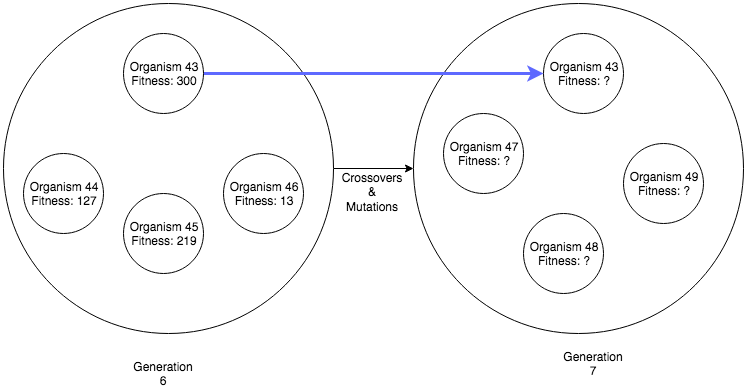
\includegraphics[scale=0.5]{elitism.png}
	\caption{Elitisme d'une génération vers la suivante}
\end{center}
\end{figure}

\subsection{Déroulement de l'algorithme}

L'organigramme ci-dessous décrit le comportement global de l'algorithme. La fonction random(0, 1) va tirer un nombre aléatoire entre compris dans l'interval $[0, 1[$. L'algorithme va donc répéter tant que la solution n'est pas optimale les étapes décrites ci-dessus pour générer des populations s'améliorant à chaque itération. Nous remarquons notamment la présence de l'élitisme ("Copy best organism to the next generation"), du principe de sélection (fonction select(...)) des crossovers (fonction crossover(p1, p2)) et des mutations (fonction mutate). 

\afterpage{%
\begin{figure}[H]
\centering
\vspace*{-3cm}
\thispagestyle{empty}
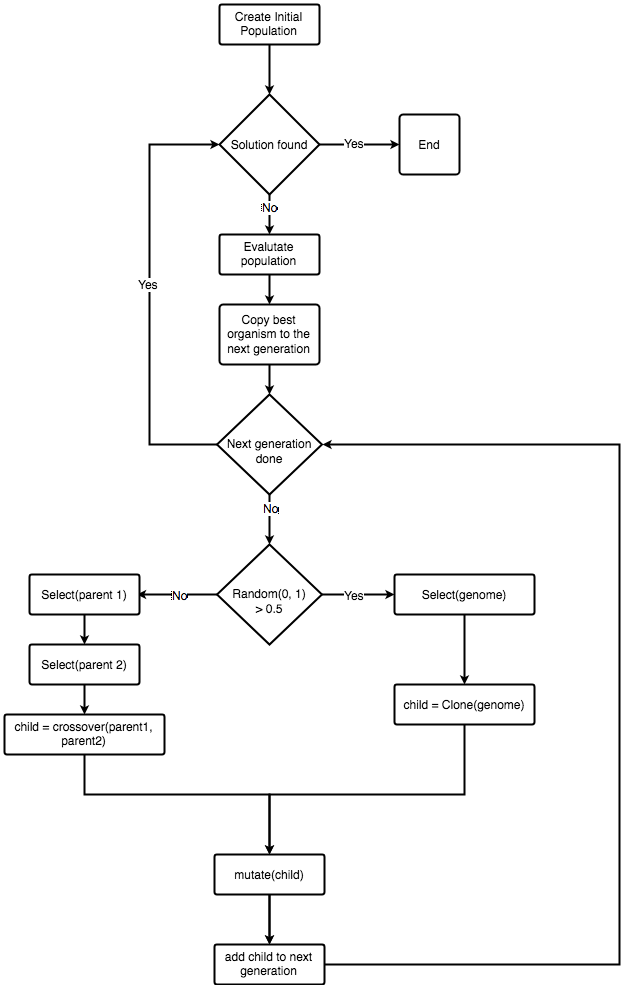
\includegraphics[scale=0.6]{mlporga.png}
\caption{Organigramme de l'algorithme naïf}
\end{figure}
\clearpage
}
\newpage

\section{NEAT}

Ce chapitre parle de l'autre algorithme de neuroévolution mis en place, NEAT (Neuroevolution of Augmenting Topologies), créé par Ken Stanley à Université du Texas à Austin. Cet algorithme détaille comment obtenir des réseaux de neurones dont la topologie change au fil des évolutions.\\
Il apporte trois techniques essentielles à son fonctionnement: suivre l'évolution des gènes avec un historique pour permettre les crossover parmi les différentes topologies, séparer les organismes en espèces afin de préserver les innovations topologiques (évolution de la structure du réseau) et faire évoluer les topologies de manière incrémentale en partant de structures simples afin d'obtenir des résultats minimaux\cite{wikineat}.

\subsection{Génome \& Phénome}

Dans le cas de NEAT, le génome est plus complexe que dans le cas du réseau à topologie fixe, en effet il doit représenter tous les neurones et toutes les connexions. Etant donné que le réseau n'est pas forcément entièrement connecté, et que les connexions peuvent "sauter" des couches, le génome est constitué de deux listes, une qui représente tout les neurones du réseau et une qui représente toutes les connexions du réseau. 

\begin{figure}[H]
\begin{center}
	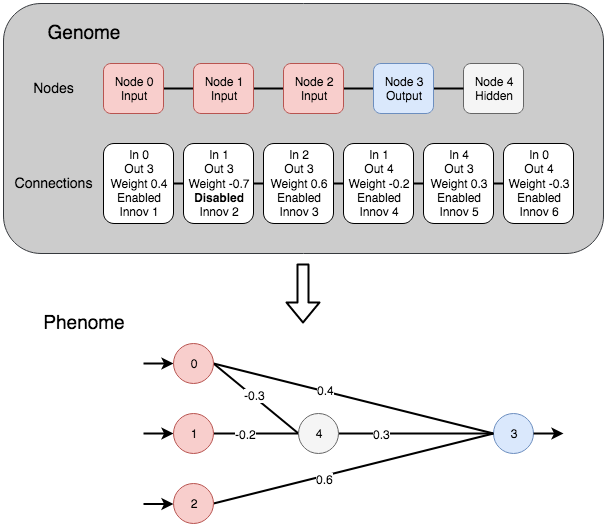
\includegraphics[scale=0.55]{genomephenomeneat.png}
	\caption{Passage du génome au phénome dans NEAT}
\end{center}
\end{figure}

\subsection{Population initiale}

La population initiale doit être aussi simple que possible, cependant il n'y a pas de règles dictant la manière dont elle doit être faite. Pour cet algorithme, la population initiale est donc un ensemble de perceptrons multicouche avec seulement une couche d'entrée et une couche de sortie dans lequel chaque entrée est reliée à chaque sortie.

\begin{figure}[H]
\begin{center}
	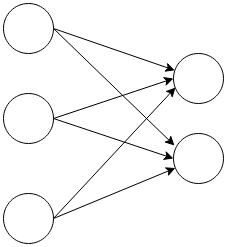
\includegraphics[scale=0.6]{initneat.png}
	\caption{Exemple de population initiale dans NEAT}
\end{center}
\end{figure}

Ce choix a été fait pour conserver un équilibre entre une population simple (pas de couche intermédiaire) mais qui est rapidement capable de s'ajuster car les connexions sont déjà disponibles. Nous ne perdons donc pas de générations uniquement pour créer les connexions.

\subsection{Historique des innovations}

Une innovation est l'apparition dans le génome d'une nouvelle connexion. Un point central de l'algorithme est de suivre l'émergence de ces innovations afin d'étiqueter les innovations semblables par un même numéro. Ainsi, si nous avons deux réseaux ayant la même topologie qui, l'un après l'autre font apparaitre une nouvelle connexion entre les mêmes neurones, leurs deux connexions auront le même numéro d'innovation.\\

Il est essentiel de faire cet étiquetage pour pouvoir ensuite reconnaitre les similarités entre les génomes notamment pour le classement en espèces et les crossover.\\
	
Afin de faire ce lien, il faut d'abord faire une recherche pour savoir si cette connexion a déjà été ajoutée dans un autre réseau. Si oui, la connexion ajoutée prend le numéro d'innovation déjà existant. Sinon un nouveau numéro d'innovation est généré et nous l'ajoutons à l'historique des innovation sous le format suivant (numéro d'innovation, neurone d'entrée, neurone de sortie, innovations déjà présentes dans le génome).\\

\subsection{Spéciation}

Une particularité de NEAT est la séparation des organismes en espèces. L'objectif de cette séparation est de protéger les nouvelles topologies pour qu'elles ait le temps de se développer et de pénaliser les espèce ne s'améliorant pas avec le temps.\\ 

Pour effectuer cette spéciation, il faut comparer les similarités entre les génomes, plus particulièrement il faut aligner les gènes homologues (ayant le même numéro d'innovation) et compter les gènes dit \textit{disjoints} où \textit{excess}.\\
Un gène est dit disjoint s'il n'apparait que dans un des deux génomes comparés mais que son numéro d'innovation est plus petit que le plus grand numéro d'innovation de l'autre génome. Un gène est dit excess s'il n'apparait que dans un des deux génomes comparés mais que son numéro d'innovation est plus grand que le plus grand numéro d'innovation de l'autre génome. Les gènes qui ne sont ni disjoints ni excess sont dit \textit{matching}.

\begin{figure}[H]
\begin{center}
	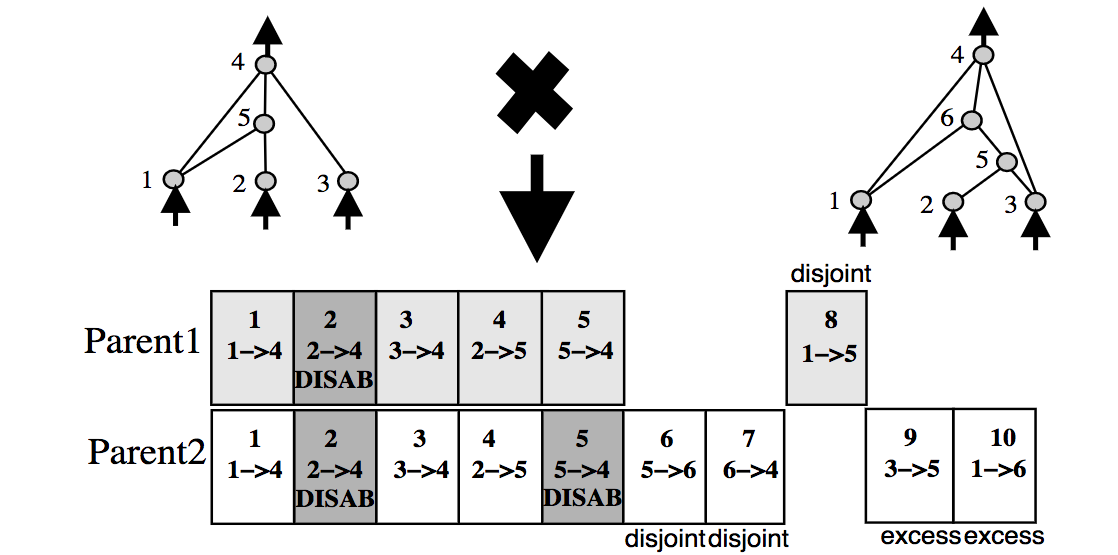
\includegraphics[scale=0.4]{disjointexcess.png}
	\caption{Comparaison de deux génomes dans NEAT\cite{neatpaper}}
\end{center}
\end{figure}

La dernière étape avant de pouvoir calculer la distance entre deux génomes est de calculer la moyenne des écarts entre les poids de chaque connexion.
La formule calculant la disparité entre deux génomes est la suivante:

\begin{equation}
	\delta = \frac{c_1 \cdot E}{N} + \frac{c_2 \cdot D}{N} + c_3 \cdot \overline{W}
\label{eq:delta}
\end{equation}

Où\\
$c_1$ est le coefficient d'excess\\
$E$ est le nombre de gènes excess\\
$c_2$ est le coefficient de disjoints\\
$D$ est le nombre de gènes excess\\
$N$ est le nombre total de gènes, peut être assigné à 1 si le réseau est petit (moins de 20 connexions)\\
$c_3$ est le coefficient de l'écart des poids\\
$\overline{W}$ est la moyenne des écarts des poids\\

Les coefficients peuvent être modifiés pour changer la sensibilité de la classification aux différents paramètres. Une fois la valeur de $\delta$ calculée, elle est comparée avec un seuil $\delta_t$, si la valeur est plus grande, les génomes ne font pas partie de la même espèce, sinon ils font partie de la même espèce.\\

Afin de préserver l'innovation et d'éviter qu'une espèce ne domine rapidement la totalité de la population, ce qui entrainerai une diminution de la variété des solutions et confinerai l'algorithme dans une petite partie de l'espace de recherche, un mécanisme de \textit{fitness sharing} est mis en place. Pour ce faire, le fitness de chaque organisme d'une espèce est divisé par le nombre d'organismes dans cette espèce. Ainsi, les petites espèces qui émergent d'une innovation topologique seront protégées de l'extinction pendant quelques génération afin de laisser le temps aux organismes de s'ajuster.\\

Plus formellement le fitness ajusté de l'organisme $i$ $f^\prime_i$ est défini comme:

\begin{equation}
	f^\prime_i = \frac{f_i}{\sum^n_{j=1} sh(\delta(i,j))}
\end{equation}
Où\\
$f_i$ est le fitness non ajusté de l'organisme i\\
$n$ est le nombre d'organismes\\
$sh$ est la fonction de sharing, celle si renvoie 0 quand son paramètre est inférieur à $\delta_t$ et 1 sinon\\
$\delta$ est la fonction comparant les génomes vue dans l'équation \ref{eq:delta}\\

\subsection{Sélection}

Dans NEAT, la sélection intervient au moment de la création d'une nouvelle génération. Cette sélection va d'abord être effectuée sur les espèce, en effet les organismes faisant partie de la moitié la moins performante de chaque espèce vont être supprimés.\\
Ensuite les espèces dont le meilleur organisme ne s'est pas amélioré depuis 15 générations sont supprimées.\\
Pour finir chaque espèce $i$ se voit attribuer un nombre d'enfants $n_i$ calculé selon la formule suivante:
\begin{equation}
	n_i = \left\lfloor\frac{\overline{sf_i}}{pop \cdot \sum^m_{j=1} \overline{sf_j}}\right\rfloor
\end{equation}
Où\\
$\overline{sf_i}$ est la moyenne des fitness des organismes de l'espèce i\\
$m$ est le nombre d'espèces\\
$pop$ est le nombre total d'organismes\\

Si le nombre d'enfants d'une espèce est inférieur à un, l'espèce disparait. Sinon l'espèce va produire n enfants dans la génération suivante en utilisant le principe de la sélection proportionnelle au fitness. En effet lors de la création d'un enfant il y a 25\% de chance que l'enfant soit une copie d'un parent sélectionné et 75\% de chance que l'enfant soit le fruit d'un crossover entre deux parents sélectionnés (il subira dans les deux cas une potentielle mutation).

\subsection{Crossover}

Le crossover dans NEAT est fait pour palier au problème des conventions concurrentes (competing conventions). En effet il est possible que deux réseaux produisent le même résultat mais de manière différente, le risque est que lorsque nous croisons les deux réseaux nous perdions une partie de l'information qui les rend efficaces.

\begin{figure}[H]
\begin{center}
	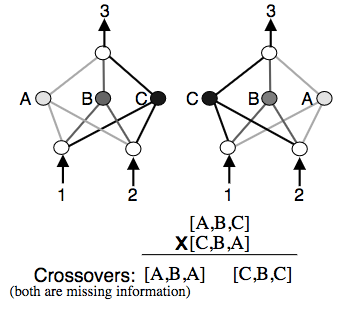
\includegraphics[scale=0.7]{competingconventions.png}
	\caption{Problème des conventions concurrentes, les deux réseaux atteignent le même résultat mais leurs possibles enfants n'auront que 2/3 de l'information \cite{neatpaper}}
	\label{fig:competing}
\end{center}
\end{figure}

En effet la figure \ref{fig:competing} nous montre deux réseau organisés différemment mais tout deux composés des mêmes éléments (A, B et C). Cependant si nous alignons de manière naïve les deux génome pour les croiser, leurs enfants seront soit [A,B,A] (il manque l'information C) soit [C,B,C] (il manque l'information A). Il est donc très probable que le résultat de ce croisement soit moins efficace que ses parents. 

Pour palier à ce problème, il faut que seuls les éléments qui divergent entre deux génomes soient échangés et que les éléments similaires soient conservés.\\

Le crossover dans NEAT se fait en alignant tous les gènes homologues (ayant le même numéro d'innovation). Pour chaque gène aligné il faut choisir aléatoirement de prendre celui du parent 1 ou du parent 2. Pour les gènes disjoint ou excess, seuls ceux du parent ayant le fitness le plus élevé sont conservés.

\begin{figure}[H]
\begin{center}
	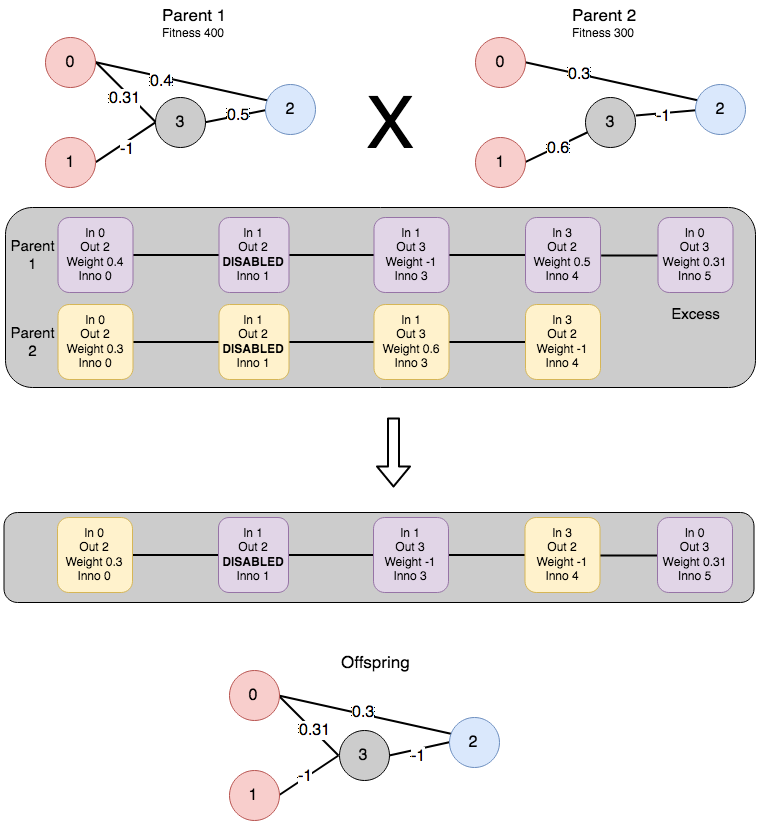
\includegraphics[scale=0.5]{crossoverneat.png}
	\caption{Crossover dans NEAT}
\end{center}
\end{figure}

\subsection{Mutation}

Les mutations dans NEAT peuvent être de trois types différents. Les pourcentages de chances que chaque mutation se produisent sont libre, cependant la publication originale de NEAT propose des valeurs qui ont montrés de bon résultats, ce sont ces valeurs qui ont été implémentées.

\subsubsection{Mutation de poids}

Une mutation de poids à 80\% de chance de se produire, si c'est le cas, tout les poids du réseau vont subir une mutation. Il y a 10\% de chance que le poids change totalement, la nouvelle valeur est donc un nombre aléatoire choisi entre -1 et 1. Les 90\% de chance restant vont faire varier le poids très légèrement, la valeur va donc subir une perturbation située entre $-0.025$ et $+0.025$.

\subsubsection{Mutation de connexion}

Une mutation de connexion consiste en l'ajout d'une connexion entre deux neurones n'étant pas déjà connectés et ne faisant pas partie de la même couche. Ce type de mutation à 5\% de chance de se produire.

\begin{figure}[H]
\begin{center}
	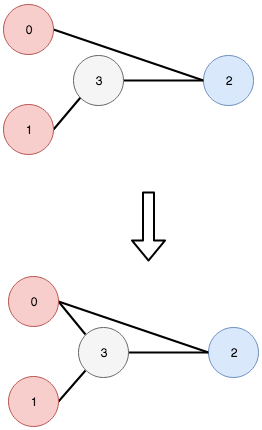
\includegraphics[scale=0.4]{addlink.png}
	\caption{Ajout d'une connexion}
\end{center}
\end{figure}

\subsubsection{Mutation de neurone}

Une mutation de neurone va ajouter un neurone dans le réseau, pour ce faire il faut choisir une connexion qui va être désactivée afin de la remplacer par deux connexions qui passent par le neurone ajouté. Cette mutation à 3\% de chance de se produire.

\begin{figure}[H]
\begin{center}
	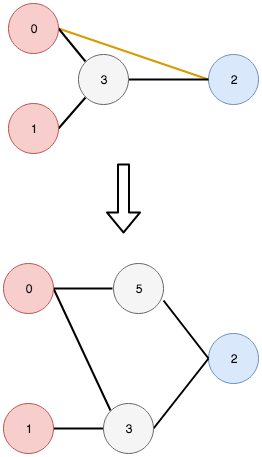
\includegraphics[scale=0.4]{addnode.png}
	\caption{Ajout d'un neurone}
\end{center}
\end{figure}

\subsection{Elitisme}

L'élitisme intervient dans l'algorithme car chaque espèce ayant au moins un enfant à créer va d'abord copier son champion de la génération passée sans lui faire subir de mutation vers la génération suivante.

\subsection{Déroulement de l'algorithme}

L'organigramme de l'algorithme NEAT se présente comme suit, il n'est pas possible de représenter en détaille toutes les opérations faites, ce diagramme montre uniquement une vue globale de l'algorithme. La fonction random(0, 1) va tirer un nombre aléatoire entre compris dans l'interval $[0, 1[$. Nous retrouvons dans l'organigramme les points vu ci-dessus notamment la spéciation ("Speciate population" et "share fitness"), la sélection ("kill bad organisms", "kill bad species", "Kill stale species" et "select"),  l'élitisme ("copy best organism"), le crossover ("crossover") et la mutation ("mutate").
\afterpage{%
\begin{figure}[H]
\centering
\vspace*{-3cm}
\thispagestyle{empty}
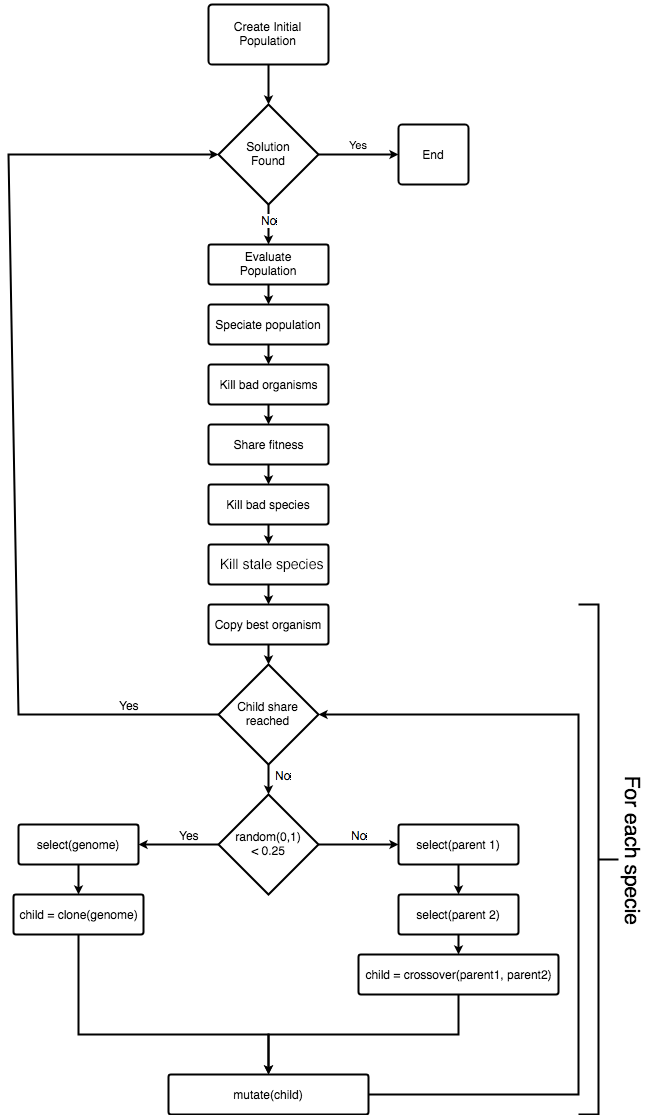
\includegraphics[scale=0.6]{neatflow.png}
\caption{Organigramme de l'algorithme NEAT}
\end{figure}
\clearpage
}
\newpage

\section{Architecture Réseau}

Cette section détaille le système distribué mis en place pour le projet et l'architecture de ces composants.

\subsection{Motivation}

La mise en place d'un système distribué basé sur une architecture client-serveur a été effectuée afin d'optimiser la vitesse de calcul. Le but est d'exploiter la puissance de calcul de plusieurs machines en parallèle. Les clients effectuent les simulations demandées et le serveur gère les génomes et s'occupe de distribuer de manière équitable le travail entre tout les clients.\\

\begin{figure}[H]
\begin{center}
	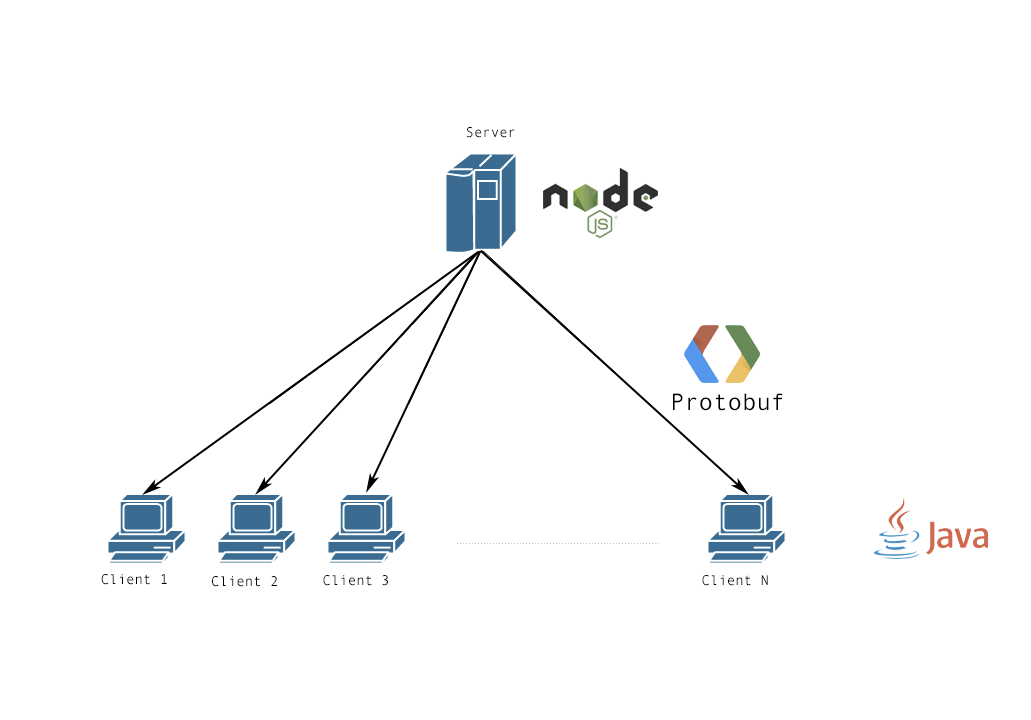
\includegraphics[scale=0.5]{archnet.png}
	\caption{Architecture réseau}
\end{center}
\end{figure}

\subsection{Serveur}

Comme écrit ci-dessus, le serveur à la lourde tâche de gérer tous les génomes et leurs fitness afin de mettre en oeuvre les algorithmes évolutionniste qui vont permettre l'évolution. En plus de cela il va également devoir servir les pages web servant à la gestion et à la surveillance du processus évolutif et répondre au requêtes sur l'API.\\
Afin de pouvoir effectuer toutes ces tâches, le serveur est constitué de modules node.js qui vont chacun gérer une partie de ce qui est lui est demandé.\\
L'architecture se présente ainsi:
\begin{figure}[H]
\begin{center}
	\includegraphics[scale=0.5]{"server.png"} 
	\caption{Architecture des modules du serveur}
\end{center}
\end{figure}

Le module server.js contient le point d'entrée du serveur, ainsi que les callbacks en cas de requêtes web / API.\\

Le module mgnetwork.js gère les communications web entre le serveur et les clients.\\

Le module pool.js gère la tâche en cours et s'occupe de la distribution des génomes aux clients.\\

Le module client.js donne une abstraction d'un client.\\

Le module genetic.js donne une interface générique pour les algorithmes génétiques, les fonctions disponibles sont:

\begin{itemize}
	\item \texttt{createRandomPopulation} qui va générer une population initiale selon l'algorithme passé en paramètres.
	\item \texttt{metadataFromTopology} qui va générer une chaine de caractères représentant les hyperparamètres d'un réseau.
	\item \texttt{genomeString} qui va convertir un génome dans une représentation sous la forme d'une chaine de caractères.
	\item \texttt{createNextGeneration} qui va utiliser le bon algorithme évolutionniste pour créer la génération suivante.
\end{itemize}

\inputminted[breaklines,breaksymbol=, frame=single,label=Genetic functions, stepnumber=1,tabsize=2]{javascript}{genetic.js}

Le module neat.js gère la totalité de l'algorithme NEAT.\\

Le module mlp.js gère la totalité de l'algorithme naïf.\\

\subsection{Client}

Le client va devoir effectuer la simulation demandée par le serveur avec le bon réseau de neurones afin d'obtenir le fitness de ce réseau. Pour ce faire il a fallu définir un format pour l'envoi d'un génome par le serveur qui puisse être transformé en réseau de neurones par le client.\\
Ce format est constitué de deux éléments, la métadonnée du réseau qui est une chaine de caractères représentant le topologie du réseau. Ainsi que le génome qui va donner les informations sur le connexions, les poids etc...\\

La métadonnée est encodée dans un format simple: "\#entrées,\#couche cachées,\#neurones couche 1,\#neurones couche 2,...,\#sorties". Par exemple soit un réseau à topologie fixe avec 8 entrées, 2 couches cachées, la première avec 6 neurones, la deuxième avec 4 neurones et enfin 4 sorties. La métadonnée sera "8,2,6,4,4".\\

L'encodage du génome dépends du type de réseau, pour les réseaux à topologie fixe, il s'agit simplement de la liste des poids à appliquer sur le réseau. Dans le cas d'un réseau de l'algorithme NEAT l'encodage est plus complexe: "\#connexions,\#neurones,id du biais,\#couches,entrée de la connexion 0,sortie de la connexion 0,poids de la connexion 0,...,neurone 0, couche du neurone 0,...".

\begin{figure}[H]
\begin{center}
	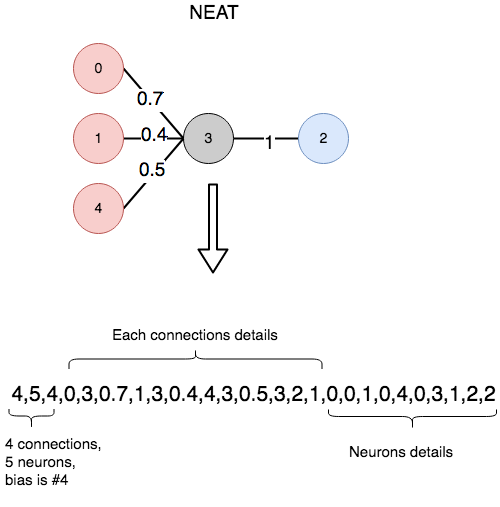
\includegraphics[scale=0.5]{neatgenomecode.png}
	\caption{Encodage du réseau NEAT}
\end{center}
\end{figure}

\subsubsection{Réseaux de neurones}

Les réseau de neurones sont utilisés de manière transparente via une class abstraite laissant paraitre un constructeur minimaliste et deux fonction, une pour propager un signal dans le réseau de neurones, l'autre pour afficher le réseau de neurones.

 \inputminted[breaklines,breaksymbol=, frame=single,label=Neural network, stepnumber=1,tabsize=2]{java}{nn.java}
 
Cette classe est ensuite héritée par deux autres classes, une pour le réseau à topologie fixe et l'autre pour le réseau NEAT. La classe \texttt{GenomeCodec} se charge du décodage des génomes et de la création des réseau de neurones via la fonction \texttt{toNeuralNetwork}.

 \inputminted[breaklines,breaksymbol=, frame=single,label=Genome Codec, stepnumber=1,tabsize=2]{java}{codec.java}

Les fonctions d'activations sont représentées par l'interface \texttt{ActivationFunction}. Les fonctions step, sigmoid et tanh sont implémentés dans la classe \texttt{ActivationFunctions}.

 \inputminted[breaklines,breaksymbol=, frame=single,label=Activation Functions, stepnumber=1,tabsize=2]{java}{activation.java}
 
 Etant donné que les types des fonctions et leurs paramètres sont compatibles avec la définition de l'interface, l'accès à ces fonctions peut être fait par référence (p.ex \texttt{ActivationFunctions::Sigmoid}). 


\subsubsection{Simulateur}

Le simulateur va permettre au réseau de neurones de jouer au jeu demandé et calculer son fitness pendant la partie de jeu.\\

Les simulateurs sont représentés par une interface, ainsi chaque jeu pouvant être simulé devra implémenter l'interface et notamment la fonction \texttt{simulate} qui va effectuer la totalité de la simulation puis renvoyer le fitness obtenu par le génome testé.
\inputminted[breaklines,breaksymbol=, frame=single,label=Simulator, stepnumber=1,tabsize=2]{java}{simulator.java}

La simulation peut également être affichée en temps réel pour avoir une visualisation du comportement de l'organisme testé. Cette visualisation est notamment affichée lorsque le client est mode spectateur

\subsubsection{Ouvrier / Spectateur}

Le client possède deux modes de fonctionnement, le mode ouvrier dans lequel il va recevoir des génomes et les évaluer dans un simulateur avant de renvoyer le fitness obtenu au serveur, et le mode spectateur. Dans ce mode le client va recevoir de la part du serveur le meilleur génome de chaque génération évaluée afin que le client affiche le résultat obtenu. En mode spectateur le client n'est donc pas chargé de faire de calculs de fitness, il est uniquement utile pour observer l'évolution.

\subsubsection{Lancement}

Le programme reçois ses paramètres depuis les arguments de la ligne de commande. Le format de la commande de lancement est le suivant: \texttt{java -jar client.jar <server\_ip> <nb\_threads> <client\_name>}. Pour démarrer le client en mode spectateur, il suffit de rajouter l'option \texttt{-s} en fin de ligne. Le fait de configurer le programme en ligne de commande permet de déployer de manière assez simple via ssh.  

\subsubsection{Multithreading}

Le client est un programme multithreadé, en effet nous pouvons choisir au lancement de démarrer autant de client en simultané que nous le désirons. Aux yeux du serveur chaque thread est un client à part, ils vont donc tous recevoir différents génomes qu'ils testeront de manière séparée avant de renvoyer indépendamment les résultat au serveur. Le choix du nombre de threads se fait au lancement du programme.

\subsubsection{Tests}

Afin de s'assurer du bon fonctionnement des réseaux de neurones, un package de test a été crée, ce dernier contient deux fichier qui vont tester les deux types de réseau de neurones sur leur capacité à effectuer un ou exclusif (XOR) avec les bons paramètres.

\subsection{Protocole}

Le protocole à été établi à l'aide du langage protobuf (Protocol Buffers). Ce dernier a été développé par Google, il permet d'avoir une définition claire ne dépendant pas des langages dans lesquels le protocole est ensuite implémenté.\\

Le compilateur protoc permet d'obtenir un ficher de gestion en Java pour le coté client et un en JavaScript (node) pour le coté serveur. Ainsi nous avons une interface pour permettre la communication entre les deux technologies.\\

Avant d'être envoyés sur le réseau, les messages doivent d'abort être sérialisés dans un format TLV (type, longueur, valeur). Le type sera l'identifiant du type du message (un byte), la longueur sera la longueur du message généré par protobuf (quatre bytes) et la valeur sera le message encodé par protobuf\cite{protobuf}.\\

Voici le fichier qui défini le protocole dans le syntaxe proto2:
\inputminted[breaklines,breaksymbol=, frame=single,label=Protocole, stepnumber=1,tabsize=2]{protobuf}{mg.proto}

Le protocole définit donc 6 types de messages:
\begin{itemize}
\item MG\_JOIN, Envoyé par le client, c'est une demande à rejoindre le groupe de calcul. En paramètres sont donnés le nom du client et si il veut rejoindre en tant que spectateur ou non.
\item MG\_JOIN\_RESPONSE, Envoyé par le serveur, confirme ou infirme l'ajout au groupe du client. Il n'existe pour l'instant aucune raison pour le rejet d'un client.
\item MG\_COMPUTE\_REQUEST, Envoyé par le serveur, demande au client de calculer le fitness d'un génome donné sur un jeu donné.
\item MG\_COMPUTE\_RESPONSE, Envoyé par le client, indique au serveur si oui ou non le client est en mesure d'effectuer la simulation.
\item MG\_COMPUTE\_RESULT, Envoyé par le client, donne le fitness obtenu par le génome donné dans le message MG\_COMPUTE\_REQUEST sur le jeu donné dans ce même message et le temps (ms) pris par le client pour effectuer la simulation.
\item MG\_END, Envoyé par n'importe quel entité, indique un désir de terminer la connexion.\\
\end{itemize}

Voici un exemple de communication entre le serveur et un client:
\begin{figure}[H]
\begin{center}
	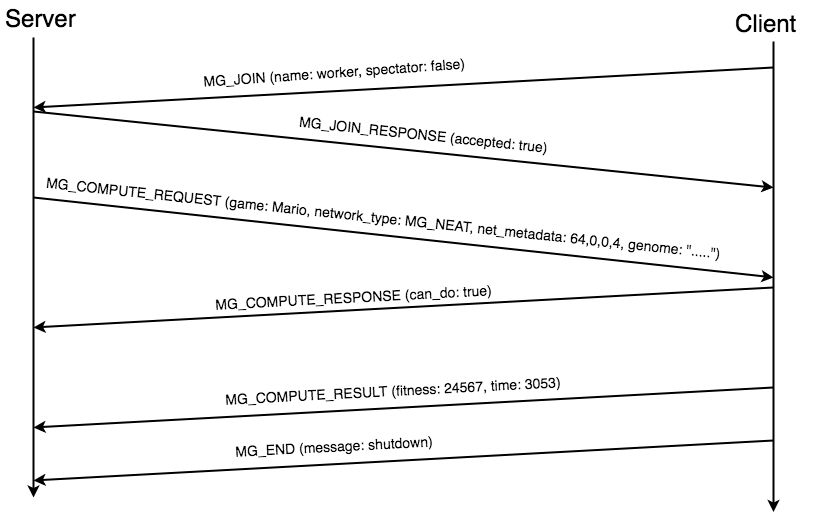
\includegraphics[scale=0.5]{sequence.png} 
	\caption{Communication Client-Serveur}
\end{center}
\end{figure}


\newpage
\section{Interface de Controle}

Cette section décrit brièvement le fonctionnement de l'interface permettant de contrôler le fonctionnement du système.\\

Cette interface web servie par le serveur permet de contrôler la tâche à effectuer. Le serveur utilise le language de templating pug (anciennement jade) pour générer la page de contrôle. L'accès à cette page se fait en faisant une requête à l'adresse du serveur sur le port 8080.\\

\subsection{Mode}

La première partie de la page de contrôle concerne le mode de fonctionnement du serveur. Le formulaire permet de choisir sur quel jeu  nous voulons entraîner les réseaux de neurones (seul le jeu Asteroid est disponible pour le moment), le type d'algorithme à employer (NEAT ou MLP) et la topologie du réseau à entraîner.

\begin{figure}[H]
\begin{center}
	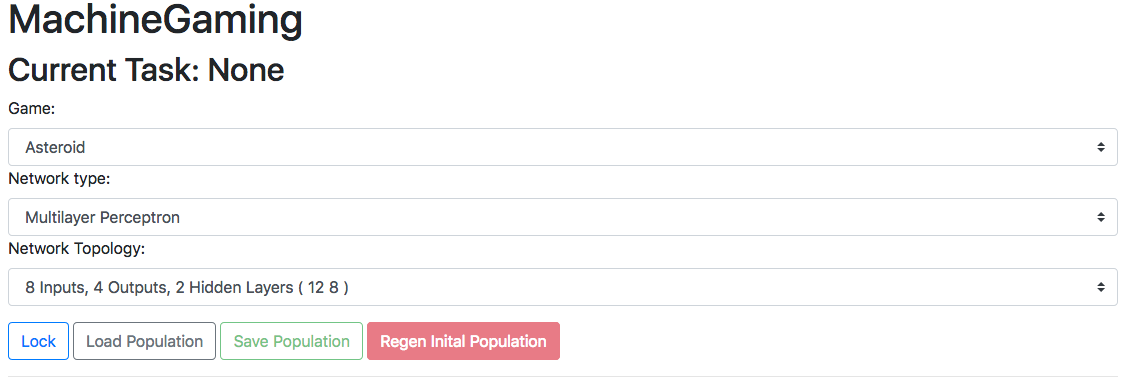
\includegraphics[scale=0.4]{unlockedmode.png} 
	\caption{Formulaire de choix de mode}
\end{center}
\end{figure}

Une fois le mode de fonctionnement choisi, nous pouvons verrouiller ce choix en appuyant sur "Lock". 

\begin{figure}[H]
\begin{center}
	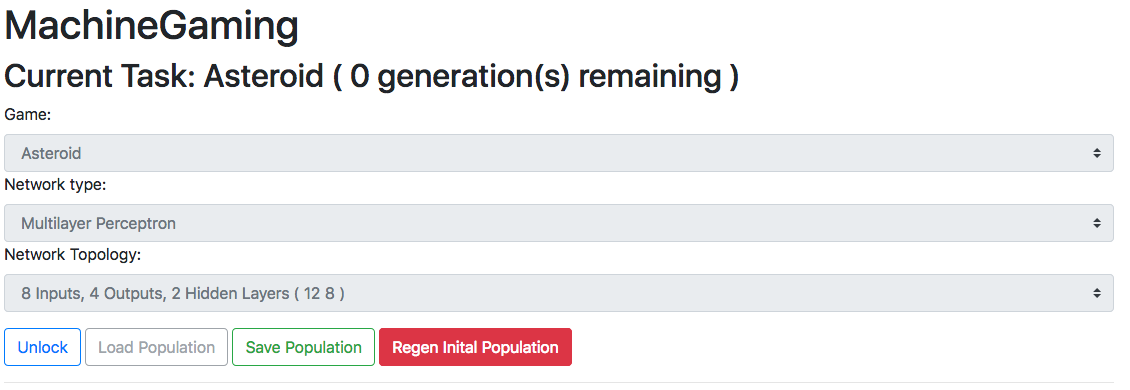
\includegraphics[scale=0.4]{lockedmode.png} 
	\caption{Formulaire de choix de mode verrouillé}
\end{center}
\end{figure}

Le bouton "Save Population", cliquable uniquement en mode verrouillé sert à sauvegarder l'état d'une population afin de reprendre le travail plus tard. La population se voit assigner un numéro unique, basé sur l'epoch UNIX.\\

Le bouton "Load Population", cliquable uniquement en mode déverrouillé sert à charger une sauvegarde d'une ancienne tâche. Pour ce faire une fenêtre modale s'affiche et il faut choisir le numéro de l'ancienne sauvegarde (les numéros sont triés par ordre chronologiques).\\

\begin{figure}[H]
\begin{center}
	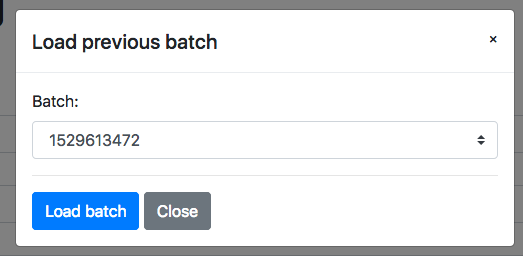
\includegraphics[scale=0.4]{loadpop.png} 
	\caption{Fenêtre de choix pour le chargement d'une population}
\end{center}
\end{figure}

Le bouton "Regen Initial Population", cliquable uniquement en mode verrouillé permet de recréer une population aléatoire, anéantissant donc tout les progrès effectués. 

\subsection{Tâche}

La gestion de la tâche se fait via la série de boutons suivante:
\begin{figure}[H]
\begin{center}
	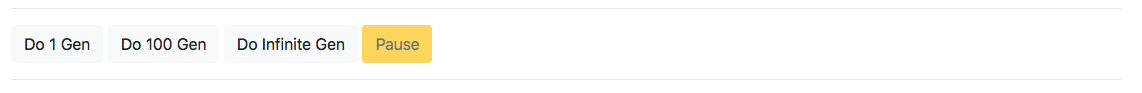
\includegraphics[scale=0.4]{taskmgr.png} 
	\caption{Boutons de gestion de la tâche}
\end{center}
\end{figure}

Le bouton "Do 1 Gen" va démarrer une génération d'évolution, le bouton "Do 100 Gen" va démarrer 100 générations d'évolution, le bouton "Do Infinite Gen" va démarrer une infinité de génération d'évolutions.\\

Le bouton "Pause" va attendre la fin de la génération en cours puis interrompre la tâche en cours. Il est impossible de déverrouiller le mode de fonctionnement ou de démarrer une nouvelle tâche tant qu'une tâche est en cours d'execution il faut donc soit attende la fin de la tâche ou la mettre en pause.

\subsection{Ouvriers}

La suite de la page affiche des cartes représentant les ouvriers, sur cette carte s'affiche le nom donné au client, son identifiant (numéro unique) et son état actuel (Waiting si le client est en attente de recevoir des ordres, Computing si le client est en train d'effectuer une simulation).

\begin{figure}[H]
\begin{center}
	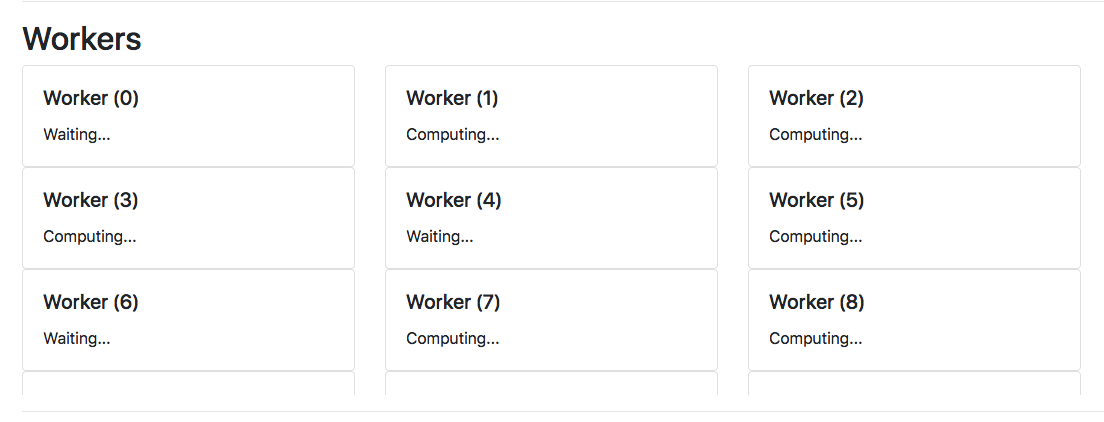
\includegraphics[scale=0.4]{workers.png} 
	\caption{Affichage des ouvriers sur l'interface de controle}
\end{center}
\end{figure}


\subsection{Graphiques}

La dernière partie de l'interface de contrôle présente deux graphiques, le premier montre l'évolution du fitness moyen par génération, le second montre le meilleur fitness de chaque génération. Ces deux graphiques se rafraichissent automatiquement et montrent uniquement les 50 dernières générations afin de ne pas saturer l'image.

\begin{figure}[H]
\begin{center}
	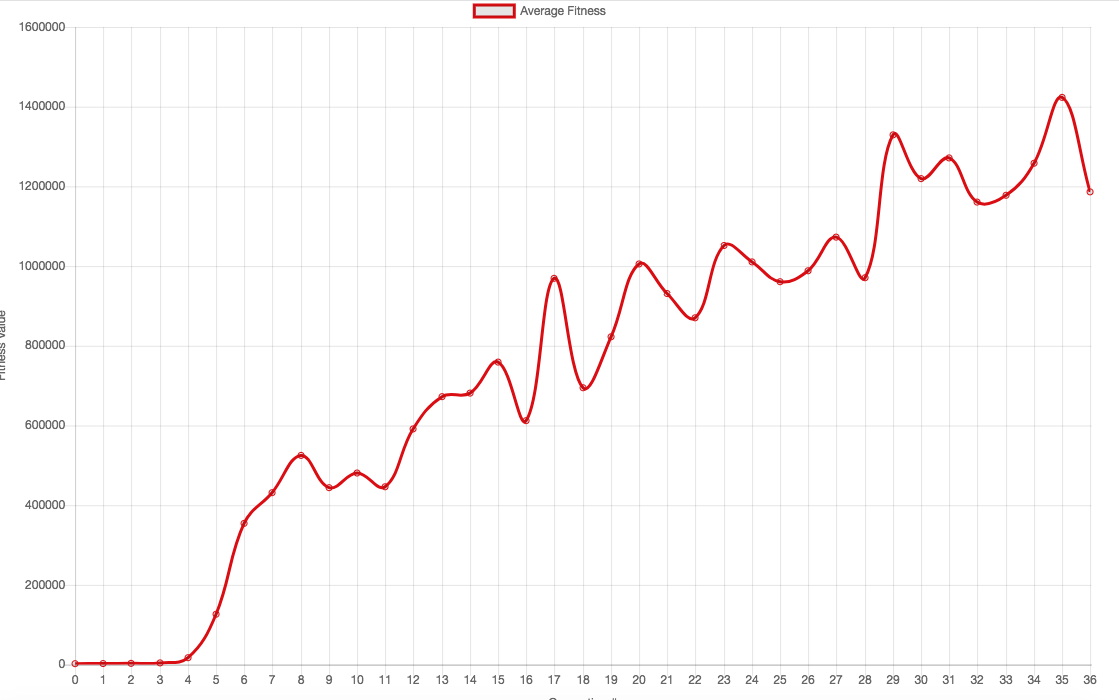
\includegraphics[scale=0.3]{avgfitgraph.png}
	\caption{Graphique des fitness moyens}
\end{center}
\end{figure}

\begin{figure}[H]
\begin{center}
	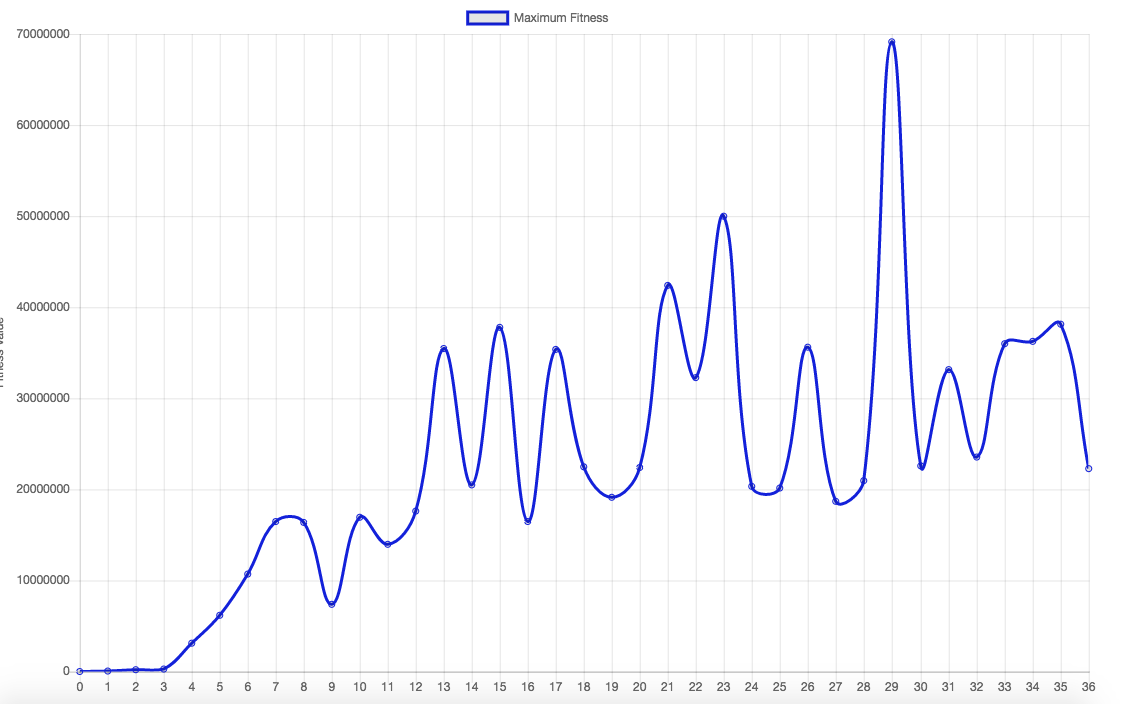
\includegraphics[scale=0.3]{maxfitgraph.png}
	\caption{Graphique des meilleurs fitness}
\end{center}
\end{figure}

\newpage
\section{Base de données}

Ce chapitre décrit le système de base de données mis en place pour  permettre la sauvegarde et le chargement des évolutions précédentes.\\

Le technologie choisie est MongoDB, cette technologie de base de données NoSQL orientée document permet le stockage sans schéma prédéfini de volumes important d'informations\cite{wikimongo}.\\

L'accès à la base de données ce fait uniquement par le serveur, celui-ci utilise le module node.js Mongoose pour effectuer les requêtes vers la base de données.\\

Le stockage des informations se fait sous le format suivant:
\begin{verbatim}
    batchId: Number,
    genNumber: Number,
    topoID: Number,
    avgFitnesses: [Number],
    bestFitnesses: [Number],
    genomes: [String],
    species: [{
        bestFitness: Number,
        best: String,
        staleness: Number,
        averageFitness: Number
    }],
    innovationHistory: [{
        from: Number,
        to: Number,
        innovationNumber: Number,
        innovationNumbers: [Number]
    }]	
\end{verbatim}

Dans le cas de l'algorithme naïf, les champs \texttt{species} et \texttt{innovationHistory} seront vide. Cependant il est essentiel de les sauvegarder dans le cadre de NEAT car sans eux l'évolution serai corrompue si elle est reprise après une sauvegarde. 

\newpage
\section{API}

Cette section décrit le fonctionnement de l'API mise en place afin de permettre une implémentation personnalisée de l'interface de contrôle. Ainsi par le biais de quelques requêtes il est possible d'obtenir toutes les informations sur l'évolution et de contrôler la tâche à effectuer.\\

\subsection{GET /status}

Une requête \texttt{get} sur la route \texttt{/status} permet d'obtenir les informations sur le serveur.\\

Le retour de la requête sera au format JSON, la structure est la suivante:
\inputminted[breaklines,breaksymbol=, frame=single,label=Status, stepnumber=1,tabsize=2]{javascript}{status.js}

\subsection{GET /saves}

Une requête \texttt{get} sur la route \texttt{/saves} permet d'obtenir les toutes les sauvegardes disponnibles dans la base de données. Les sauvegarde sont au format défini dans le section 9.\\

\subsection{POST /work}
Une requête \texttt{post} sur la route \texttt{/work} permet de définir le mode de fonctionnement du serveur.\\

Si le paramètre \texttt{lock} est défini, la requête est une demande de verrouiller ou de déverrouiller le mode de fonctionnement.\\

Dans le cas du verrouillage, il faut spécifier l'identifiant du jeu à verrouiller dans le paramètre \texttt{tgame} (la liste des jeu est accessible dans /status), le type de réseau à utiliser (0 = MLP et 1 = NEAT, ces valeurs sont définies dans le protocole) dans le paramètre \texttt{tnet} et l'identifiant de la topologie dans le paramètre \texttt{ttopo} (la liste des topologies est également accessible dans /status).\\

Dans le cas du déverrouillage aucuns paramètre n'est nécessaire.\\

Si le paramètre \texttt{save} est défini, la requête est une demande de sauvegarder l'état de l'évolution. Aucuns autres paramètres n'est nécessaire.\\

Si le paramètre \texttt{load} est défini, la requête est une demande de charger une ancienne évolution. Dans ce cas le paramètre \texttt{lbatch} doit être défini comme l'identifiant de la sauvegarde à charger (la liste des sauvegardes est accessible dans /saves).\\

Si le paramètre \texttt{regen} est défini, la requête est une demande de recréation de la population initiale.

\subsection{POST /task}

Une requête \texttt{post} sur la route \texttt{/task} permet de définir la tâche à effectuer.\\

Si le paramètre \texttt{pause} est défini, la requête est une demande de mise en pause de la tâche en cours.\\

Si le paramètre \texttt{onegen} est défini, la requête est une demande d'évolution sur une génération.\\

Si le paramètre \texttt{hungen} est défini, la requête est une demande d'évolution sur 100 générations.\\

Si le paramètre \texttt{infgen} est défini, la requête est une demande d'évolution sur une infinité de générations.\\

\newpage
\section{Jeux}

Ce chapitre explique le fonctionnement de l'évolution d'agents apprenant à jouer à un jeu vidéo. Le seul jeu implémenté pendant le réalisation de ce projet est le jeu d'arcade Asteroids. Cependant l'architecture du projet permet l'ajout d'autres jeux facilement.

\subsection{Asteroids}

Le jeu Asteroids original à été crée en 1979 par Atari sous la forme d'une borne d'arcades. Le concept du jeu est très simple, le joueur contrôle un vaisseau spatial triangulaire et doit éviter les astéroïdes qui errent sur l'écran.\\

\begin{figure}[H]
\begin{center}
	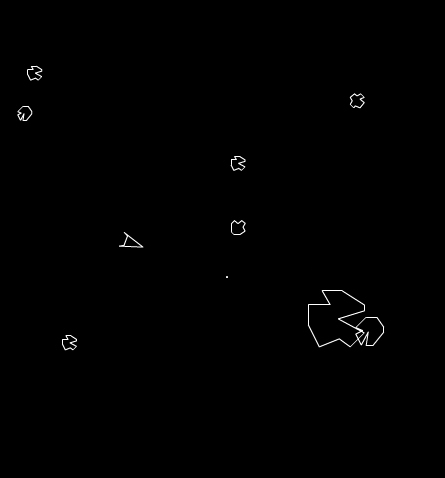
\includegraphics[scale=0.6]{game.png}
	\caption{Image du jeu Asteroids}
\end{center}
\end{figure}

Pour marquer des points, le joueur dois détruire des astéroïdes en tirant dessus. Lorsqu'un astéroïde est détruit il se divise en deux plus petits astéroïdes qui eux aussi peuvent se diviser en deux plus petits astéroïdes. Ces derniers cependant ne peuvent pas se diviser. La figure ci-dessous schématise ce concept.

\begin{figure}[H]
\begin{center}
	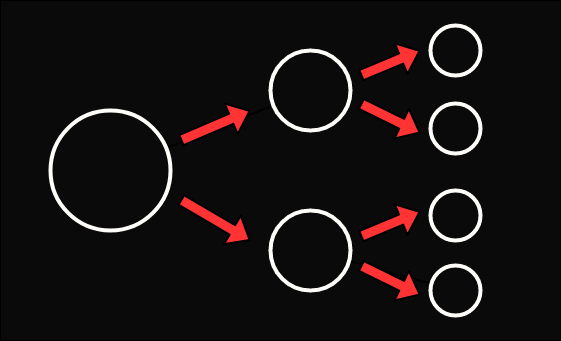
\includegraphics[scale=0.3]{asteroids.png}
	\caption{Subdivision des astéroïdes}
\end{center}
\end{figure}

La difficulté réside dans le fait que la multiplication du nombre d'astéroïde va rendre l'esquive de plus en plus difficile. De plus quand le joueur à fini de détruire les quatre premiers astéroïdes et leurs enfants, cinq nouveaux astéroïdes apparaissent aléatoirement, puis six, puis sept, etc...\\

Le vaisseau peut se déplacer vers l'avant, tourner à gauche ou à droite et tirer tout droit. Lorsque le vaisseau va de l'avant, il gagne une inertie qu'il va perdre progressivement lorsque le joueur arrête d'accélérer.

La position et la direction des astéroïdes est aléatoire. Si un objet sort par la gauche de l'écran il réapparait à droite et inversement (même chose pour le haut et le bas). Le joueur voit la totalité du monde à chaque instant du jeu et joue seul. Il s'agit donc d'un environnement continu, observable, dynamique, simple agent, non-déterministe et non-épisodique.\\

\subsubsection{Entrées}

Afin de pouvoir faire jouer un agent intelligent à ce jeu il a fallu créer des capteurs qui lui permettent de comprendre son environnement.\\

L'information qui semble la plus importante pour l'apprentissage de ce jeu est la présence d'astéroïdes autour du vaisseau. Nous allons donc vérifier dans huit directions (Nord, Nord est, Est, Sud est, Sud, Sud ouest, Ouest, Nord ouest) quel astéroïde est le plus proche et donner l'inverse de cette distance (il s'agit donc d'une valeur entre 0 et 1, 1 étant un danger imminant) à notre réseau de neurones afin d'obtenir l'action à effectuer.\\

\begin{figure}[H]
\begin{center}
	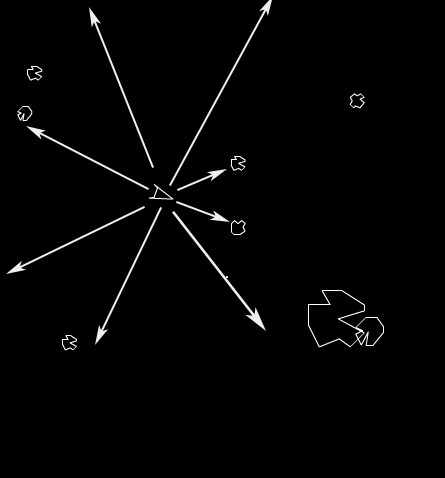
\includegraphics[scale=0.6]{sensors.png}
	\caption{Capteurs de distance}
\end{center}
\end{figure}

\subsubsection{Sorties}

Une fois que le réseau à effectué la propagation avant des entrées, ses sorties sont l'envie d'effectuer chaque action possibles (avancer, tourner à gauche, tourner à droite et tirer). Si la valeur de la sortie est supérieur à 0.8 l'action sera effectuée.

\subsubsection{Affichage}

Si le client est en mode spectateur il va afficher le jeu en temps réel, ainsi que le réseau de neurones prenant les décisions. Sur le réseau, les connexions en vert sont des connexions ayant un poids positif et les connexions en rouge sont des connexions ayant un poids négatif. 

\begin{figure}[H]
\begin{center}
	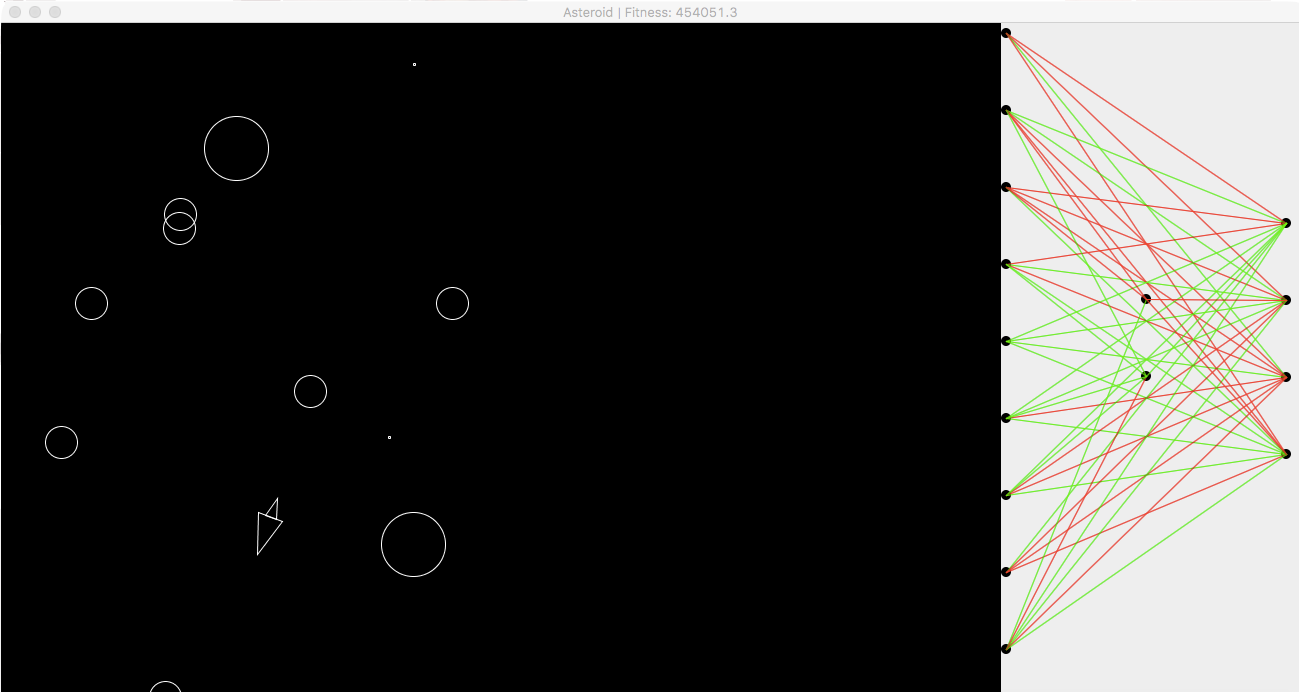
\includegraphics[scale=0.35]{spectatormode.png}
	\caption{Affichage du jeu en mode spectateur}
\end{center}
\end{figure}

\subsubsection{Fitness}

La fonction de fitness définie pour ce jeu est la suivante

\begin{equation}
	f = ticks \cdot 10 \cdot score + score \cdot (\frac{score}{shot})^2	
\end{equation}
Où\\
$ticks$ est le nombres d'instant de jeu passés (temps de surive)\\
$score$ est le nombre d'astéroïdes touchés\\
$shot$ est le nombre de coups tirés\\

\subsubsection{Résultats}

Les résultats de l'évolution sont très intéressants, en effet nous obtenons rapidement des réseau ayant appris à esquiver les astéroïdes.\\

Plus exactement l'algorithme naïf met entre 15 et 20 générations en moyenne avant d'arriver à esquiver les astéroïdes. Ce moment très clairement visible sur le graphique du fitness moyen.\\

\begin{figure}[H]
\begin{center}
	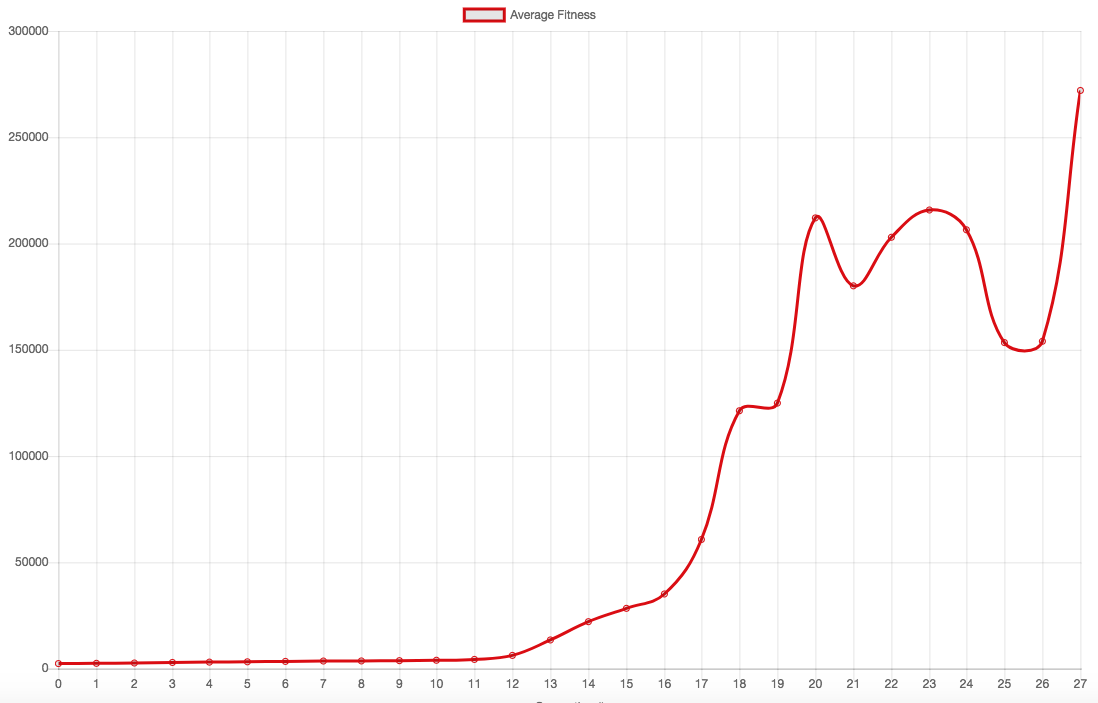
\includegraphics[scale=0.35]{mlpdodge.png}
	\caption{Fitness moyen de l'algorithme naïf, le fitness augmente rapidement autour de la génération 17 dû à l'apprentissage de l'esquive}
\end{center}
\end{figure}

Pour le NEAT l'apprentissage de l'esquive se fait bien plus tôt. En effet autour de la cinquième génération les agents savent déjà esquiver les astéroïdes bien que ce soit aux alentours de la 10ème génération que la technique est perfectionnée.

\begin{figure}[H]
\begin{center}
	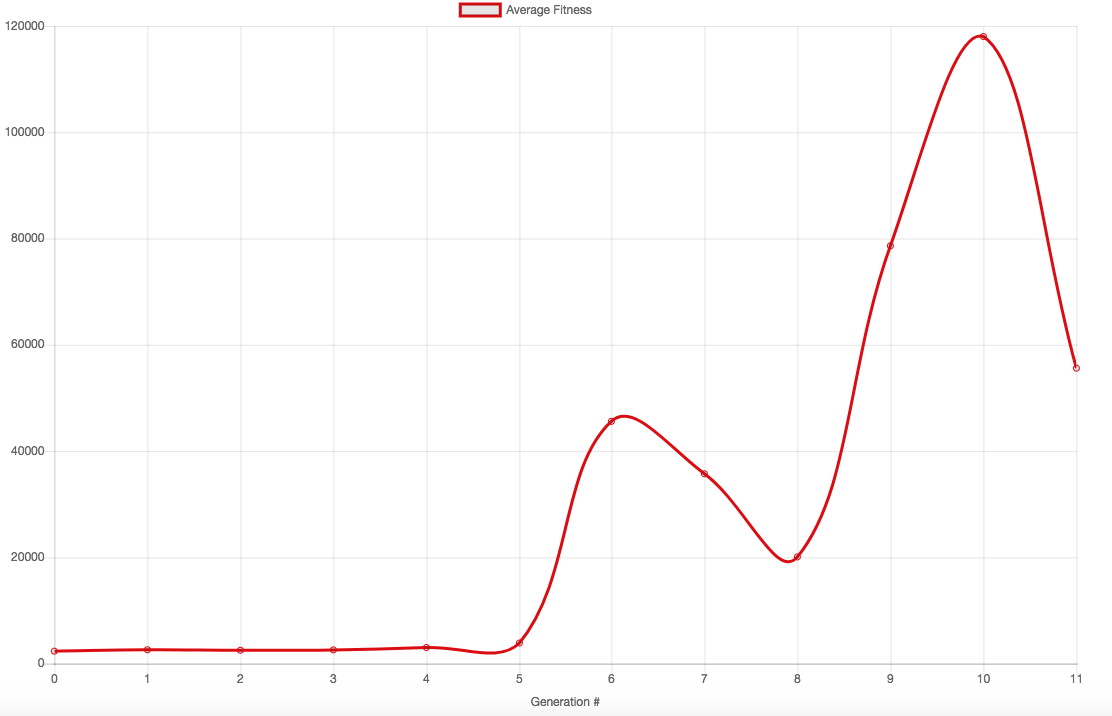
\includegraphics[scale=0.35]{neatdodge.png}
	\caption{Fitness moyen de NEAT, le fitness augmente rapidement autour de la génération 5 dû à l'apprentissage de l'esquive}
\end{center}
\end{figure}

Cependant apprendre l'esquive simple ne suffit pas car il est possible que le réseau fonce dans un astéroïde en essayant d'en esquiver un autre. La technique est donc perfectionnée petit à petit et au bout d'une centaine de générations ($\sim$5 minutes) ils sont capable d'attendre des scores très impressionnants.\\

Un phénomène intéressant est que peu importe l'algorithme utilisé, le comportement qui va se répandre le plus vite est toujours le même: tourner sur soit même. En effet ce comportement semble dominer à chaque fois. Une raison qui peut expliquer ce phénomène est que l'esquive au départ est une réaction à la présence d'un astéroïde vers le capteur situé à l'arrière du vaisseau. Ainsi tourner sur soit même va permettre de vérifier la présence d'astéroïdes dans toutes les directions et donc d'avancer si il y a un danger. Par la suite l'esquive est perfectionnée mais ce trait reste car il en est à l'origine. Une autre explication possible est le fait de compenser l'inertie, en effet lorsqu'un vaisseau fini d'accélérer (pour esquiver par exemple) il conserve une inertie qui peut s'avérer potentiellement mortelle si un astéroïde se trouve droit devant, pour compenser le vaisseau doit donc se tourner pour accélérer légèrement dans l'autre sens et s'arrêter.\\

Après 100 générations l'algorithme naïf obtient un fitness moyen d'environ 300'000, ce score correspond à des agents capables de détruire les quatre premiers astéroïdes et leurs enfants mais qui n'arrivent pas a réagir à l'apparition des cinq suivants. Cette barre des 300'000 est passée par NEAT après seulement 20 générations.\\

Après 100 générations NEAT arrive à un fitness d'environ 1'600'000, ce qui correspond à un agent capable détruire les quatre premiers astéroïdes, puis les cinq suivant, mais qui tombe face à la masse de sous-astéroïdes quand il commence à détruire les six d'après. Il est cependant peu probable qu'un agent puisse s'améliorer au delà de cette limite, en effet la précision qu'il faudrait pour manoeuvrer à travers autant d'objet n'est pas atteignable avec ce simulateur. Cette limite des 1'600'000 n'est d'ailleurs pas franchie même si système tourne pendant un jour entier.\\

\begin{figure}[H]
\begin{center}
	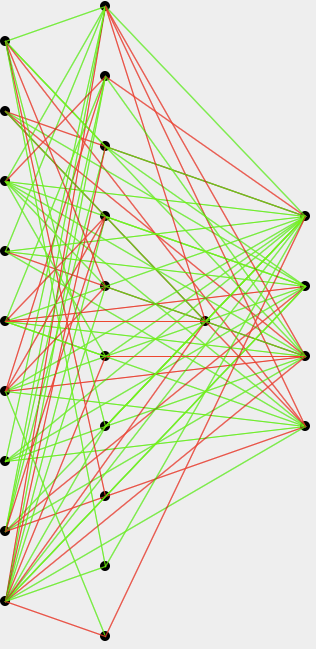
\includegraphics[scale=0.45]{neatevolv.png}
	\caption{Réseau NEAT après 50 générations}
\end{center}
\end{figure}

\newpage
\section{Conclusion}

La réalisation de ce travail durant trois mois fût une expérience extrêmement enrichissante, sur le plan personnel car gérer son temps, ses capacités de travail et sa motivation pendant un longue période était un défi mais également sur le plan technique car il a fallu faire beaucoup de recherche en amont pour avoir les bases nécessaires à la réalisation du projet et de tous ces aspect allant de l'implémentation d'un protocole réseau, la création d'un jeu vidéo, la gestion d'algorithmes évolutionnistes et de réseaux de neurones.\\

Le travail réalisé me rend fier et je suis toujours étonné par la rapidité de l'évolution de ces simples organismes artificiels progressant à vue d'oeil et développant des stratégies tellement différentes de celles qu'un humain utiliserai.\\

Entreprendre ce projet m'a permis d'explorer ce monde si vaste et passionnant qu'est celui de l'intelligence artificielle et bien que je n'ai fait qu'en écorcher la surface cela ne m'a que plus motivé à poursuivre d'autres projet dans le domaine.\\

\subsection{Suite du projet}

Ce système de neuroévolution ayant été développé de manière très généraliste, il peut facilement accueillir de nouvelles fonctionnalités. Il serait par exemple très intéressant de tester les algorithmes implémentés sur d'autres jeux, peut-être plus complexe afin de tester les limites qu'on pourrait atteindre.\\

Une autre possibilité serai d'implémenter d'autres types de réseaux de neurones tels que les CNN (réseau neuronal convolutif) ou les RNN (réseau neuronal récurrent) et de constater les différences que nous obtenons en terme de capacité d'apprentissage.

\newpage
\bibliographystyle{unsrt}
\bibliography{mg}
\end{document}
